\graphicspath{{./images/DBN_Impl/}}
\chapter{DB-nets Implementation: A CPN Tools Extension}
\label{ch:DBN_Impl}
\paragraph*{\textnormal{In this chapter, we discuss how DB-nets are modelled in CPN Tools and implemented using extension supported by CPN Tools. We develop an extension which implements the functionality of DB-nets in CPN Tools. First we provide a gentle introduction to CPN Tools extension and the framework that we adopt for implementing different aspects of DB-nets, e.g., action transitions, view places and data acquisition. Later, we present an architecture for the implementation of the different layers of DB-nets. We provide the communication pattern of our extension and briefly describe the program used for data acquisition and handling actions attached to transitions.}}
\subparagraph*{\textnormal{Considering the taxi booking example from the previous chapter, we gradually transform our CPN model to a DB-net model. We implement each of the layers independently and finally explain the connection between them. After transformation from the CPN model to the DB-net model, we can perform simulation over the transformed DB-net model.}}

\section{CPN Tools Extension}
\label{sec:DBN_Impl_CPN_Tools_Extension}
\paragraph*{\textnormal{As seen earlier, we use CPN Tools for modelling our CPN. CPN Tools has two major components:
\begin{itemize}
	\item GUI - the user interface, which provides us the functionality to model our CPNs.
	\item Simulator - which is responsible for simulation and analysis of CPNs.
\end{itemize}
The GUI of CPN Tools is written in BETA \cite{BETA} programming language and the simulator is written in SML \cite{milner1997definition}. The GUI of CPN Tools provides the functionality to draw net elements and the simulator keeps tracks of the declaration such as colour-sets and variables, ML functions, enablement and firing of transitions etc. CPN Tools (version 4) supports development of simulator extensions which help users to develop customized functionalities. Simulator extension \cite{CPN_Tools_Extension} has the possibility of adding functionalities using JAVA and also allows third parties to add functionalities without relying on BETA and SML programming languages. Simulator extensions, through JAVA programs provide control for numerous operations performed by the simulator.}}

\subsection*{Architecture}
%\label{subsec:DBN_Impl_CPN_Tools_Extension_Architecture}
\subparagraph*{\textnormal{In CPN Tools, modelling and execution of any CPN depends on the interaction between GUI and simulator (see Figure \ref{fig:DBN_Impl_CPN_Tools_Architecture}). Access/CPN \cite{AccessCPN} is a framework which facilitates the development of extensions in JAVA.
\begin{figure}[!htbp]
	\centering
	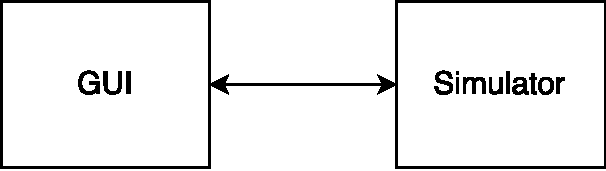
\includegraphics[scale = 0.35]{DBN_Impl_CPN_Tools_Architecture.pdf}
	\caption{Interconnectivity between CPN Tools GUI and Simulator}
	\label{fig:DBN_Impl_CPN_Tools_Architecture}
\end{figure}
Access/CPN consists of two interfaces, one is written in SML (which is close to the simulator) and the other in JAVA. The interface written in JAVA provides users with the possibility to access the simulator. Additionally the interface also provides an object oriented representation of the CPN models loaded in CPN Tools. With Access/CPN library \cite{AccessCPN_Library}, one could replace the GUI part with any component written in JAVA(see Figure \ref{fig:DBN_Impl_CPN_Tools_Architecture_Access_CPN}).
\begin{figure}[!htbp]
	\centering
	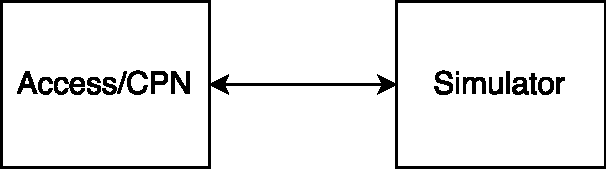
\includegraphics[scale = 0.35]{DBN_Impl_CPN_Tools_Architecture_Access_CPN.pdf}
	\caption{Interconnectivity between Access/CPN and Simulator}
	\label{fig:DBN_Impl_CPN_Tools_Architecture_Access_CPN}
\end{figure}
Using these libraries, one could develop simulator extensions in JAVA which are capable of communicating with CPN Tools Simulator and CPN Tools GUI (see Figure \ref{fig:DBN_Impl_CPN_Tools_Architecture_Extension}). The extension is directly connected with the simulator and any communication between extension and GUI takes place through the simulator. Thus, the simulator acts as a mediator between the GUI and extension.
\begin{figure}[!htbp]
	\centering
	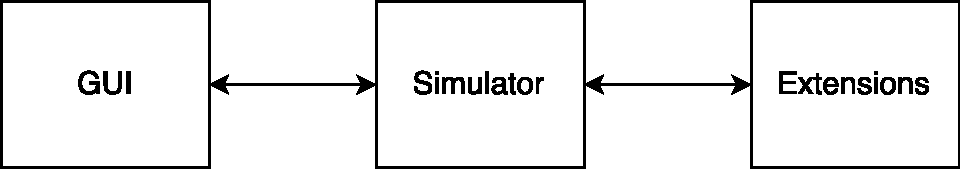
\includegraphics[scale = 0.35]{DBN_Impl_CPN_Tools_Architecture_Extension.pdf}
	\caption{Interconnectivity between GUI, Simulator and Extension}
	\label{fig:DBN_Impl_CPN_Tools_Architecture_Extension}
\end{figure}}}

\subparagraph*{\textnormal{Access/CPN provides a JAVA interface for an extension, which helps in accessing the \textit{channel} through which the communication takes place between the simulator and extension. The communication between components (GUI, simulator and extension) involves sending and receiving \textit{packets}\footnote{Packets generally contain messages in a specific format which are used to instruct the components to perform certain actions.} passing through the channel. This \textit{channel} is provided to the user in the \bsq{Extension} interface of Access/CPN. Access/CPN also provides subscription to specific events\footnote{A list of events which could be subscribed is provided in \cite{CPN_Tools_Message_Format}.} occurring in CPN Tools such as the firing of transitions, setting markings of places etc. One could listen to those events by subscribing through JAVA code (provided in the \bsq{Extension} interface of Access/CPN). Once the events are subscribed, one could \textit{handle} it (provided in the \bsq{Extension} interface of Access/CPN), and perform customised actions based on events. Various communication patterns which can be used are available in \cite{CPN_Tools_Extension}, however, for our extension, we adopt a customised communication pattern which is a mixture of patterns mentioned in \cite{CPN_Tools_Extension}.}}

\section{Comms/CPN}
\label{sec:DBN_Impl_Comms_CPN}
\paragraph*{\textnormal{Comms/CPN allows CPN Tools to communicate with external processes. Comms/CPN \cite{gallasch2001comms} is a Standard ML library that augments Design/CPN \cite{Design_CPN} with the necessary infrastructure to establish communication between CPN models and external processes. As described in \cite{Design_CPN}, Design/CPN is a tool package which supports modelling, simulation and verification by means of hierarchical CPNs. For modelling, simulation and verification purposes we already have CPN Tools and we connect it to external processes using Comms/CPN APIs. In our case, the external process is a JAVA application which is used to facilitate data acquisition and actions attached to transitions.}}

\begin{figure}[!htbp]
	\centering
	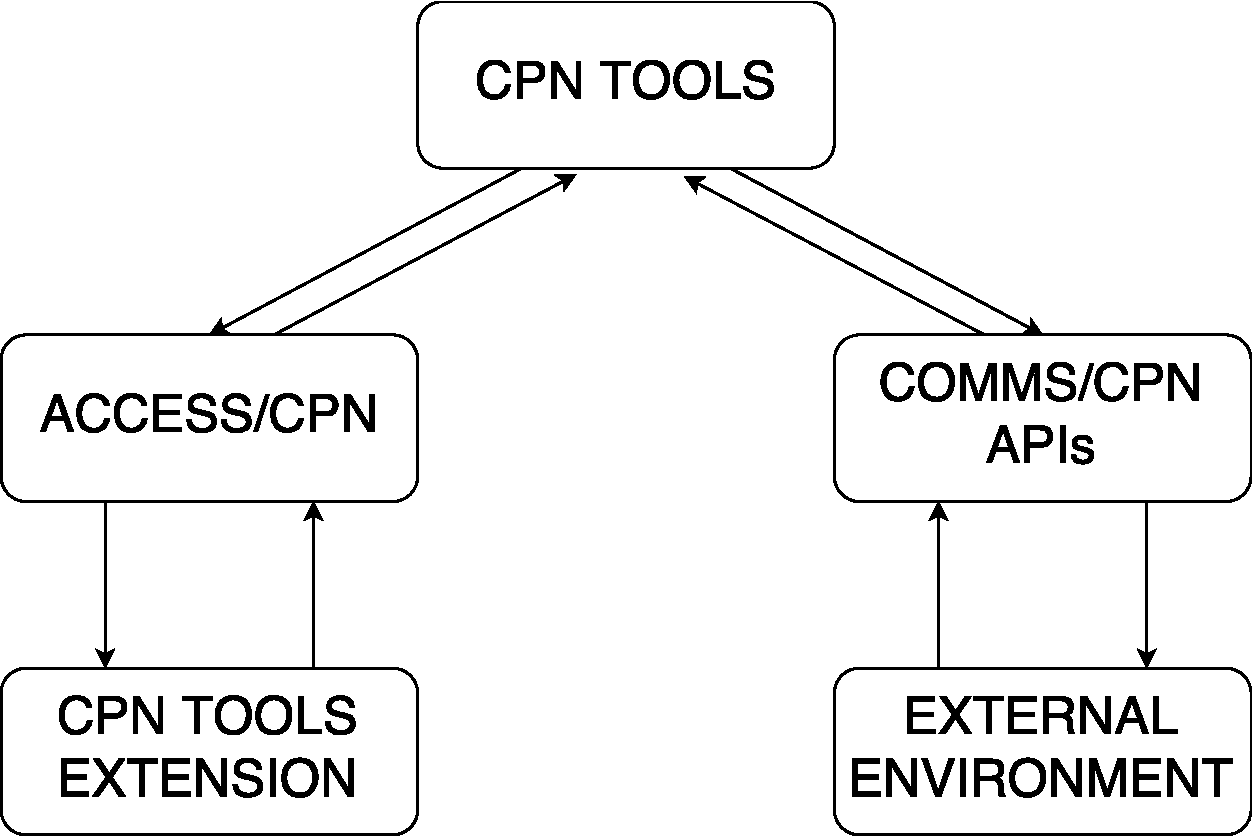
\includegraphics[scale = 0.35]{DBN_Impl_CPN_Tools_Extension_External_Environment.pdf}
	\caption{Connectivity between CPN Tools extension, external environment and CPN Tools}
	\label{fig:DBN_Impl_CPN_Tools_Extension_External_Environment}
\end{figure}

\subparagraph*{\textnormal{The Comms/CPN is implemented in a layered fashion as shown in Figure \ref{fig:DBN_Impl_COMMS_CPN_Layer} (taken from \cite{gallasch2001comms}). The topmost layer is the Connection Management Layer followed by Messaging Layer and the Communication Layer. The Comms/CPN uses TCP/IP protocol to send/receive messages in the form of stream of bytes over a specified port. Similarly, the external application connected to the specified port should also be able to send/receive messages using TCP/IP protocol. Using this architecture, Comms/CPN is able to establish communication between the CPN model and the external application.}}

\begin{figure}[!htbp]
	\centering
	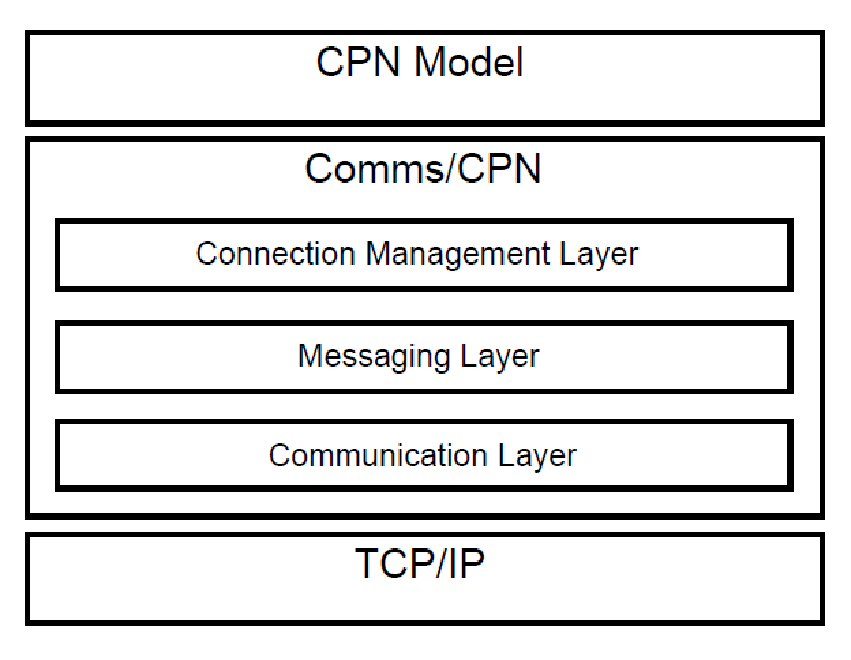
\includegraphics[scale = 0.35]{DBN_Impl_COMMS_CPN_Layer.pdf}
	\caption{Overall architecture of Comms/CPN}
	\label{fig:DBN_Impl_COMMS_CPN_Layer}
\end{figure}

\subparagraph*{\textnormal{JAVA/CPN\footnote{The source code of JAVA/CPN is provided in \cite{CPN_Tools_Comms/CPN}.}, a library written in JAVA, allows a JAVA process to communicate with Design/CPN through Comms/CPN. As mentioned in \cite{gallasch2001comms}, the current version of JAVA/CPN is the minimal implementation necessary to enable communication. Using this, one could set up a connection at a designated port and communicate with the CPN model (see Figure \ref{fig:DBN_Impl_Comms_Architecture_JAVA_CPN}).
}}
\begin{figure}[!htbp]
	\centering
	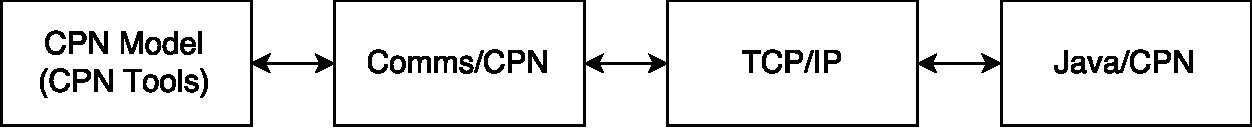
\includegraphics[scale = 0.35]{DBN_Impl_Comms_Architecture_JAVA_CPN.pdf}
	\caption{Communication between JAVA/CPN and CPN model}
	\label{fig:DBN_Impl_Comms_Architecture_JAVA_CPN}
\end{figure}

\subparagraph*{\textnormal{Comms/CPN provide a set of APIs, written in SML, namely:
\begin{enumerate}
\item \textit{openConnection} - allows users to connect to external process as a clients. It takes three parameters, the first being connection name which is a unique identifier, second is the host name and the third is a TCP/IP port number.
\item \textit{acceptConnection} - allows external processes to connect to CPN Tools GUI. It takes two parameters, first being the connection name which is a unique identifier and the second one is a TCP/IP port number.
\item \textit{send} - allows users to send any type of data to external processes. It takes three parameters, first is the connection identifier and the second is the data to be sent. The third parameter is the encoding function which is used to encode the data into a byte stream. The resultant byte stream is sent to the designated TCP/IP port. 
\item \textit{receive} - allows users to receive any type of data from external processes. It takes two parameters, first is the connection identifier followed by a parameter specifying the decoding function to  decode the received byte stream from the designated TCP/IP port.
\item \textit{closeConnection} - allows users to close a connection. Takes a single parameter which specifies the connection name to be closed.
\end{enumerate}
In our case, we do not use \textit{openConnection} API, since we do not work in a remote architecture. The messages which are sent or received, using the \textit{send} and \textit{receive} function, are in form of \textit{strings}. The \textit{closeConnection} function closes the specified connection. The JAVA/CPN library also exposes APIs, closely related to Comms/CPN and perform similar functionality, namely
\begin{enumerate}
\item \textit{connect} - requires two parameters, the hostname and the TCP/IP port.
\item \textit{accept} - requires only the port number of the TCP/IP port.
\item \textit{send} - using the encoding function, it encodes the data into a byte stream sends the byte stream to the designated TCP/IP port. 
\item \textit{receive} - receives the byte stream from the designated TCP/IP port and decodes it using the decoding function.
\item \textit{disconnect} - disconnects the connection established over the designated TCP/IP port.
\end{enumerate}}}

\subparagraph*{\textnormal{In order to make CPN Tools connect with external JAVA process, we use Connection Management Layer, which is closely connected to CPN Tools, to pass messages. The messages are then received by the processes, e.g., a JAVA process connected to the designated TCP/IP port using JAVA/CPN. In a similar fashion, messages can be sent from the JAVA application to the designated port and can be received by the CPN Tools.}}

\section{DB Nets Implementation}
\label{sec:DBN_Impl_Implementation}
\paragraph*{\textnormal{In this section, we present an idea for the implementation of different layers of DB-nets. In Figure \ref{fig:DBN_Impl_Mapping_Framework}, the DB-net layers are mapped to their corresponding implementation paradigm. The persistence layer is modelled in PostgresSQL \cite{Postgres} which is a relational database management system (RDBMS). The data logic layer is implemented as a JAVA application and for the control layer, we use CPN Tools. The JAVA application comprises our CPN Tools extension (written in JAVA) along with a JAVA process called \textit{Poll Server}, connected with JAVA/CPN, for data acquisition and executing actions.}}

\begin{figure}[!htbp]
	\centering
	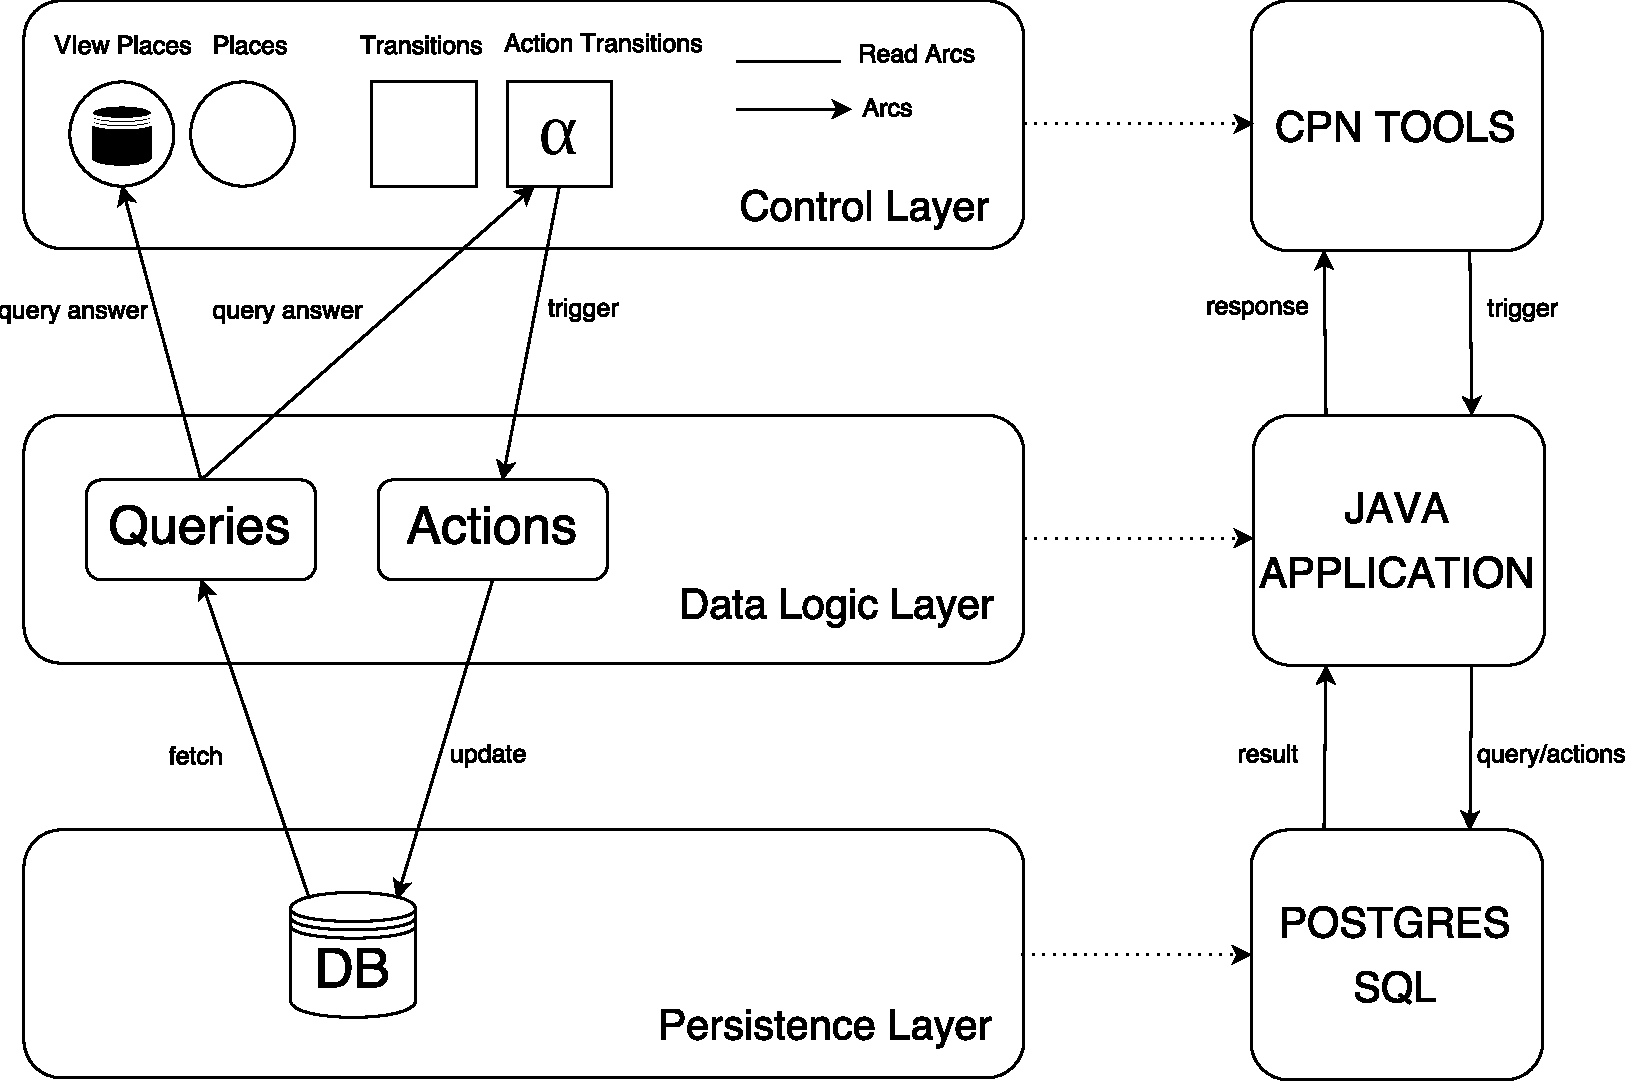
\includegraphics[scale = 0.35]{DBN_Impl_Mapping_Framework.pdf}
	\caption{The mapping of DB-net framework}
	\label{fig:DBN_Impl_Mapping_Framework}
\end{figure}

\subparagraph*{\textnormal{Figure \ref{fig:DBN_Impl_Java_App_Division} shows the framework through which the communication among different components takes place.
\begin{figure}[!htbp]
\centering
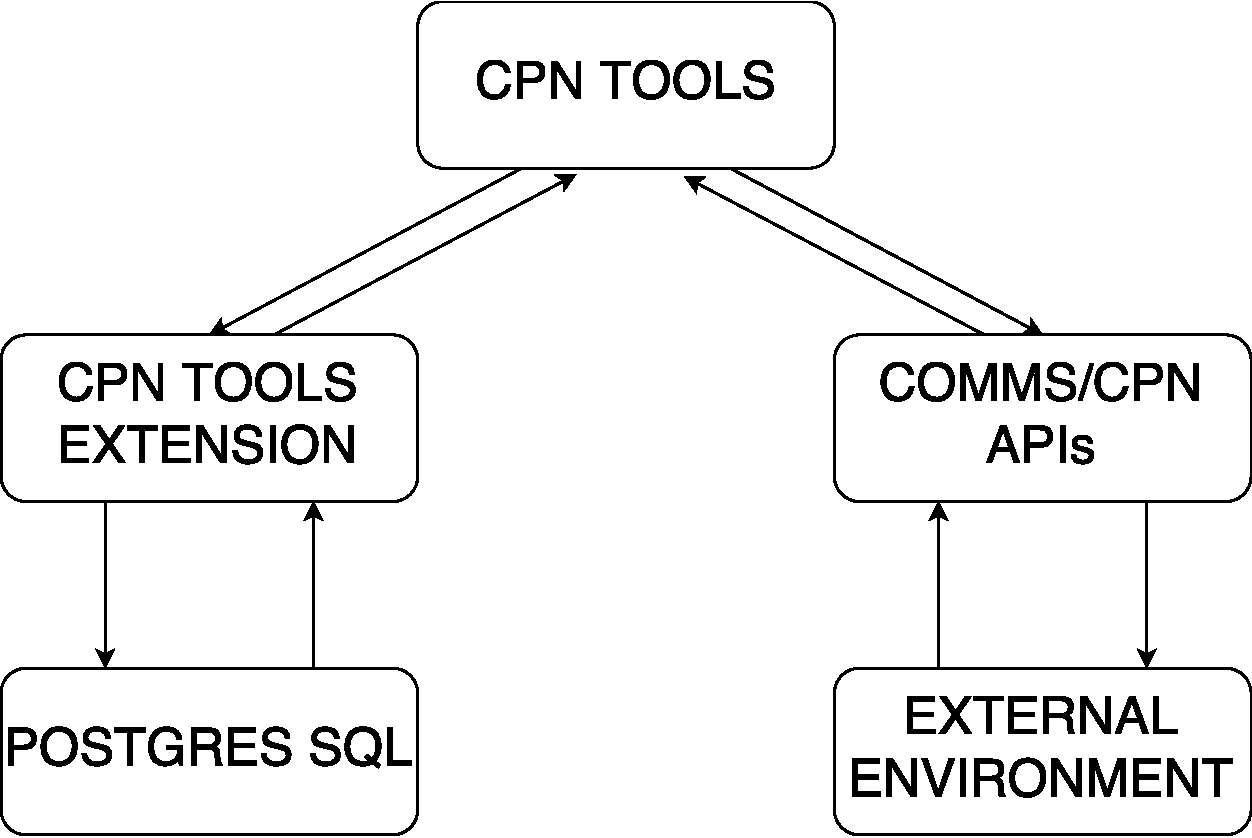
\includegraphics[scale = 0.35]{DBN_Impl_Java_App_Division.pdf}
\caption{Interconnectivity between different components}
\label{fig:DBN_Impl_Java_App_Division}
\end{figure}
Comms/CPN is used to connect to external environment/processes, which could possibly be web services etc., for data acquisition. Instead of connecting to web services, we connect to the \textit{Poll Server}.  The \textit{Poll Server} contains our JAVA functions which are used to facilitate data acquisition and executing CRUD(\textit{Create, Read, Update, Delete}) operations. The view places are populated through extension and the action transitions are executed using the \textit{Poll Server}, hence both the components are connected to the database (see Figure \ref{fig:DBN_Impl_Layer_Framework}). Connecting the \textit{Poll Server} to the database also opens up the possibility to acquire data from the database.   
\begin{figure}[!htbp]
	\centering
	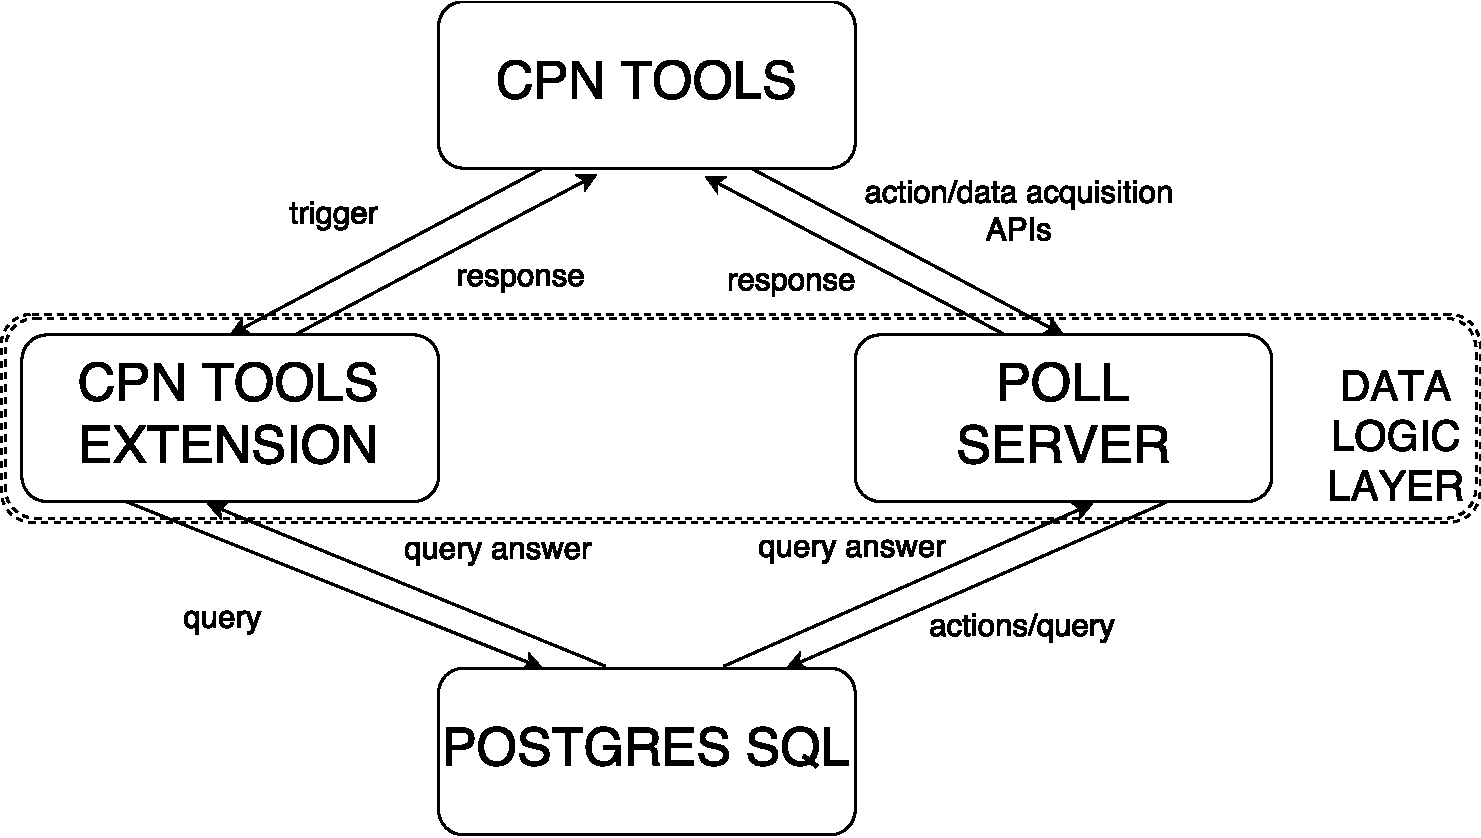
\includegraphics[scale = 0.35]{DBN_Impl_Layer_Framework.pdf}
	\caption{Data logic layer division}
	\label{fig:DBN_Impl_Layer_Framework}
\end{figure}
}}

\subsection{Persistence Layer}
\subparagraph*{\textnormal{The persistence layer consists of the database schema. We model our database schema in PostgresSQL, which allows the modelling of a full fledged relational database with constraints such as primary keys, foreign keys etc. The persistence layer is capable of returning answer to the query attached to view places along with executing actions attached to the transitions.}}

\subsection{Control Layer}
\subparagraph*{\textnormal{We use CPN Tools to implement our control layer. In CPN Tools, we define action transitions and view places which have actions and query attached to them. Let us see how to model view places and transitions in CPN Tools.}}

\subparagraph*{\textnormal{View places are drawn like normal places in CPN Tools. Also, view places carry SQL queries along themselves. Using \bsq{Text} tool one could write a statement defining the view place. Note that in the CPN model, the view places should always be connected with read arcs. The syntax\footnote{In CPN Tools, the net elements are drawn on a page which is the part of the CP net.} to define a view place is:}}
\begin{verbatim}
view_place : <PageName.PlaceName> : <SQL Query>
\end{verbatim}

\subparagraph*{\textnormal{For example, in Figure \ref{fig:DBN_Impl_Short_VP_AT_Example}, the place $\mathit{Free\ Taxi}$ has a FOL query attached. If we want to declare the place $\mathit{Free\ Taxi}$ as view place using the SQL query we could declare it as:}}

\begin{figure}[!htbp]
	\centering
	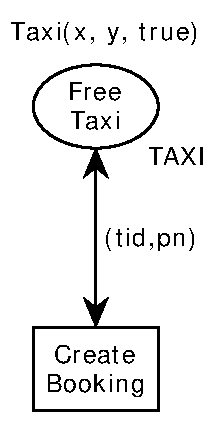
\includegraphics[scale = 0.35]{DBN_Impl_Short_VP_AT_Example.pdf}
	\caption{Example of view place}
	\label{fig:DBN_Impl_Short_VP_AT_Example}
\end{figure}

\subparagraph*{}
\begin{lstlisting}[showstringspaces=false, language = ML, caption = View place declaration example: $\mathit{Free\ Taxi}$, captionpos=b]
view_place : Booking.Free Taxi : SELECT "TID","PlateNum" FROM taxi WHERE "isFree" = TRUE;
\end{lstlisting}

\subparagraph*{\textnormal{where $\mathit{taxi}$ is the relational schema. The view place shows the details of taxis, such as taxi id and plate number, which are available for booking.}}

\subparagraph*{\textnormal{The actions attached to the transitions are modelled using ML functions. These ML functions internally use Connection Management Layer APIs provided by the Comms/CPN. As described in \cite{CPN_Tools_CodeSegment}, the code segment of transitions helps us in defining actions. The code segment has \textit{input}, \textit{output} and \textit{action} part. The input variables (the variables of interest over the incoming arc) should be mentioned in the \textit{input} part and the fresh variables, used for acquiring data, should be mentioned in the \textit{output} part. The \textit{action} part has \textit{let\ldots in \ldots end} construct which is similar to the construct of ML functions (see Listing \ref{lst:DBN_Impl_Modeling_Actions}). The fresh variables acquire data in the \textit{let} part whereas \textit{in} part contains CRUD operations. Just before the \textit{end} part, the fresh variables (if any) should be mentioned within parentheses following the order of variables in the \textit{output} part.}}

\subparagraph*{}
\begin{lstlisting}[showstringspaces=false, language = ML, caption = Code Segment: action transition, captionpos=b, label = lst:DBN_Impl_Modeling_Actions, numbers=left,
stepnumber=1]
input(<input variables>);
output(<fresh variables>);
action
let
<Data Acquisition/ Perform Actions>
in
<Perform Actions>
(<return fresh variables>)
end;
\end{lstlisting}

\subparagraph*{\textnormal{In Figure \ref{fig:DBN_Impl_Short_VP_AT_Example1}, we show the modelling of the view place $\mathit{Free\ Taxi}$ and the action transition $\mathit{Create\ Booking}$. The transition $\mathit{Create\ Booking}$ takes the free taxi and makes it unavailable for further booking. The code segment of the $\mathit{Create\ Booking}$ transition can be written as:}}

\subparagraph*{}
\begin{lstlisting}[showstringspaces=false, language = ML, caption = Code Segment: \textit{Create Booking} transition, captionpos=b, label = lst:DBN_Impl_Create_Booking_code_segment_example, numbers=left,
stepnumber=1]
input(t_id);
output();
action
let
in
RESERVE(t_id);
()
end;
\end{lstlisting}

\begin{figure}[!htbp]
	\centering
	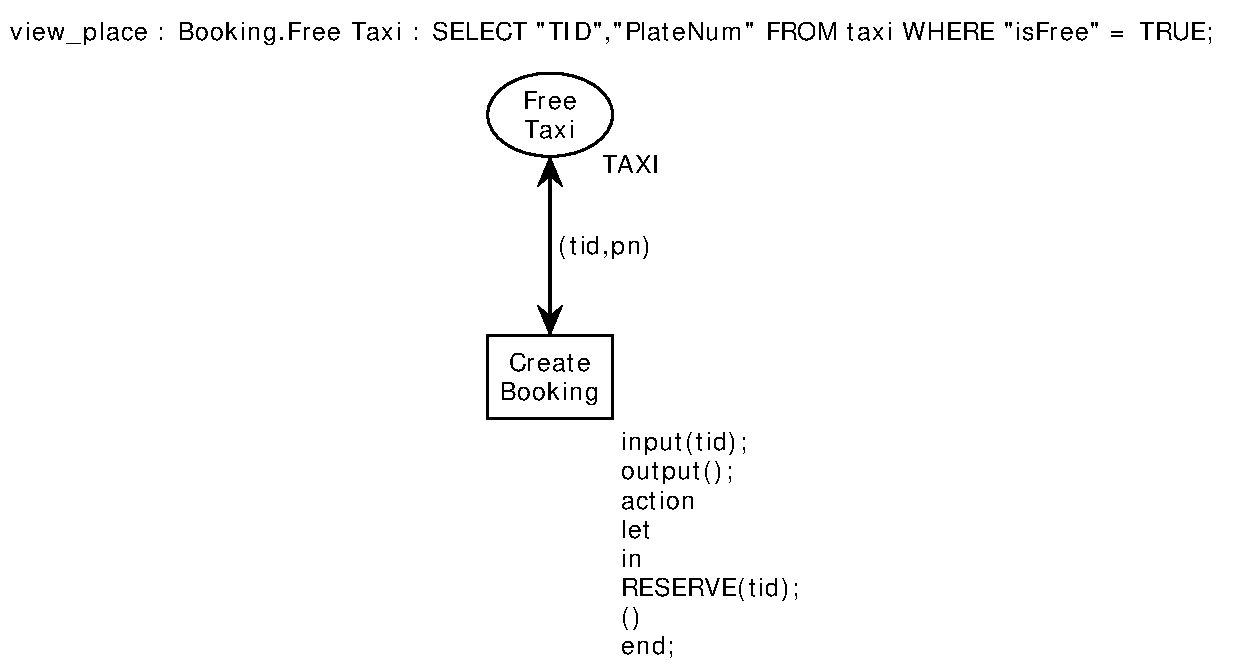
\includegraphics[scale = 0.55]{DBN_Impl_Short_VP_AT_Example_1.pdf}
	\caption{Modelling view place and action transition}
	\label{fig:DBN_Impl_Short_VP_AT_Example1}
\end{figure}

\subsection{Data Logic Layer}
\label{subsec:DBN_Impl_Implementation_Data_Logic_Layer}
\subparagraph*{\textnormal{As shown in Figure \ref{fig:DBN_Impl_Layer_Framework}, the data logic layer comprises of two parts:
\begin{itemize}
	\item A CPN Tools extension
	\item Poll Server
\end{itemize}
}}
\subsubsection*{CPN Tools extension}
\subparagraph*{\textnormal{We develop a CPN Tools extension to implement our data logic layer. With the user specified connection parameters, the extension maintains a connection with the database (Postgres SQL) using JDBC\footnote{a driver which allows JAVA application to connect to a database.} driver. The extension subscribes to CPN miscellaneous control facilities, e.g., the save event of a net, compile declarations, e.g., colour-set declaration and simulation commands, e.g., firing a transition, which are provided by CPN Tools. The main responsibilities of this extension are to:
\begin{enumerate}
\item keep track of all the net elements of the model. Also, store information about the model, such as model name, model location, pages in the net etc.
\item keep track of colour-set declarations in the CPN model. This is useful for populating the view places as we need to know the colour-set of the place before applying any marking over it.
\item keep track of the view places defined in the DB-net model, fetch the answer to the query attached to view places and calculate the markings accordingly.
\item interact with the simulator to check if the calculated markings are compatible with the colour-set the view places.
\item update the GUI on each occurring step in the simulation.
\end{enumerate}
The communication between simulator, GUI and extensions is based on packet forwarding mechanism. The communication takes place over a channel which carries the packets. Subscription to an interested event results in a notification, in form of a packet, to which we send a response. For example, once the view place is declared and the database connection is established, it results in a notification to the extension and consequently, the marking is fetched from the database and the view place is updated.}}

\subparagraph*{\textnormal{Using callback messages \cite{CPN_Tools_Callback_Messages}, one could update the GUI. In this case, a packet, including the desired update for the GUI, has to be created and passed over the channel. Note that passing invalid packets over the channel may lead CPN Tools into an inconsistent state. We design our extension on the communication pattern shown in Figure \ref{fig:DBN_Impl_Extension_Communication_Pattern}.
\begin{figure}[!htbp]
	\centering
	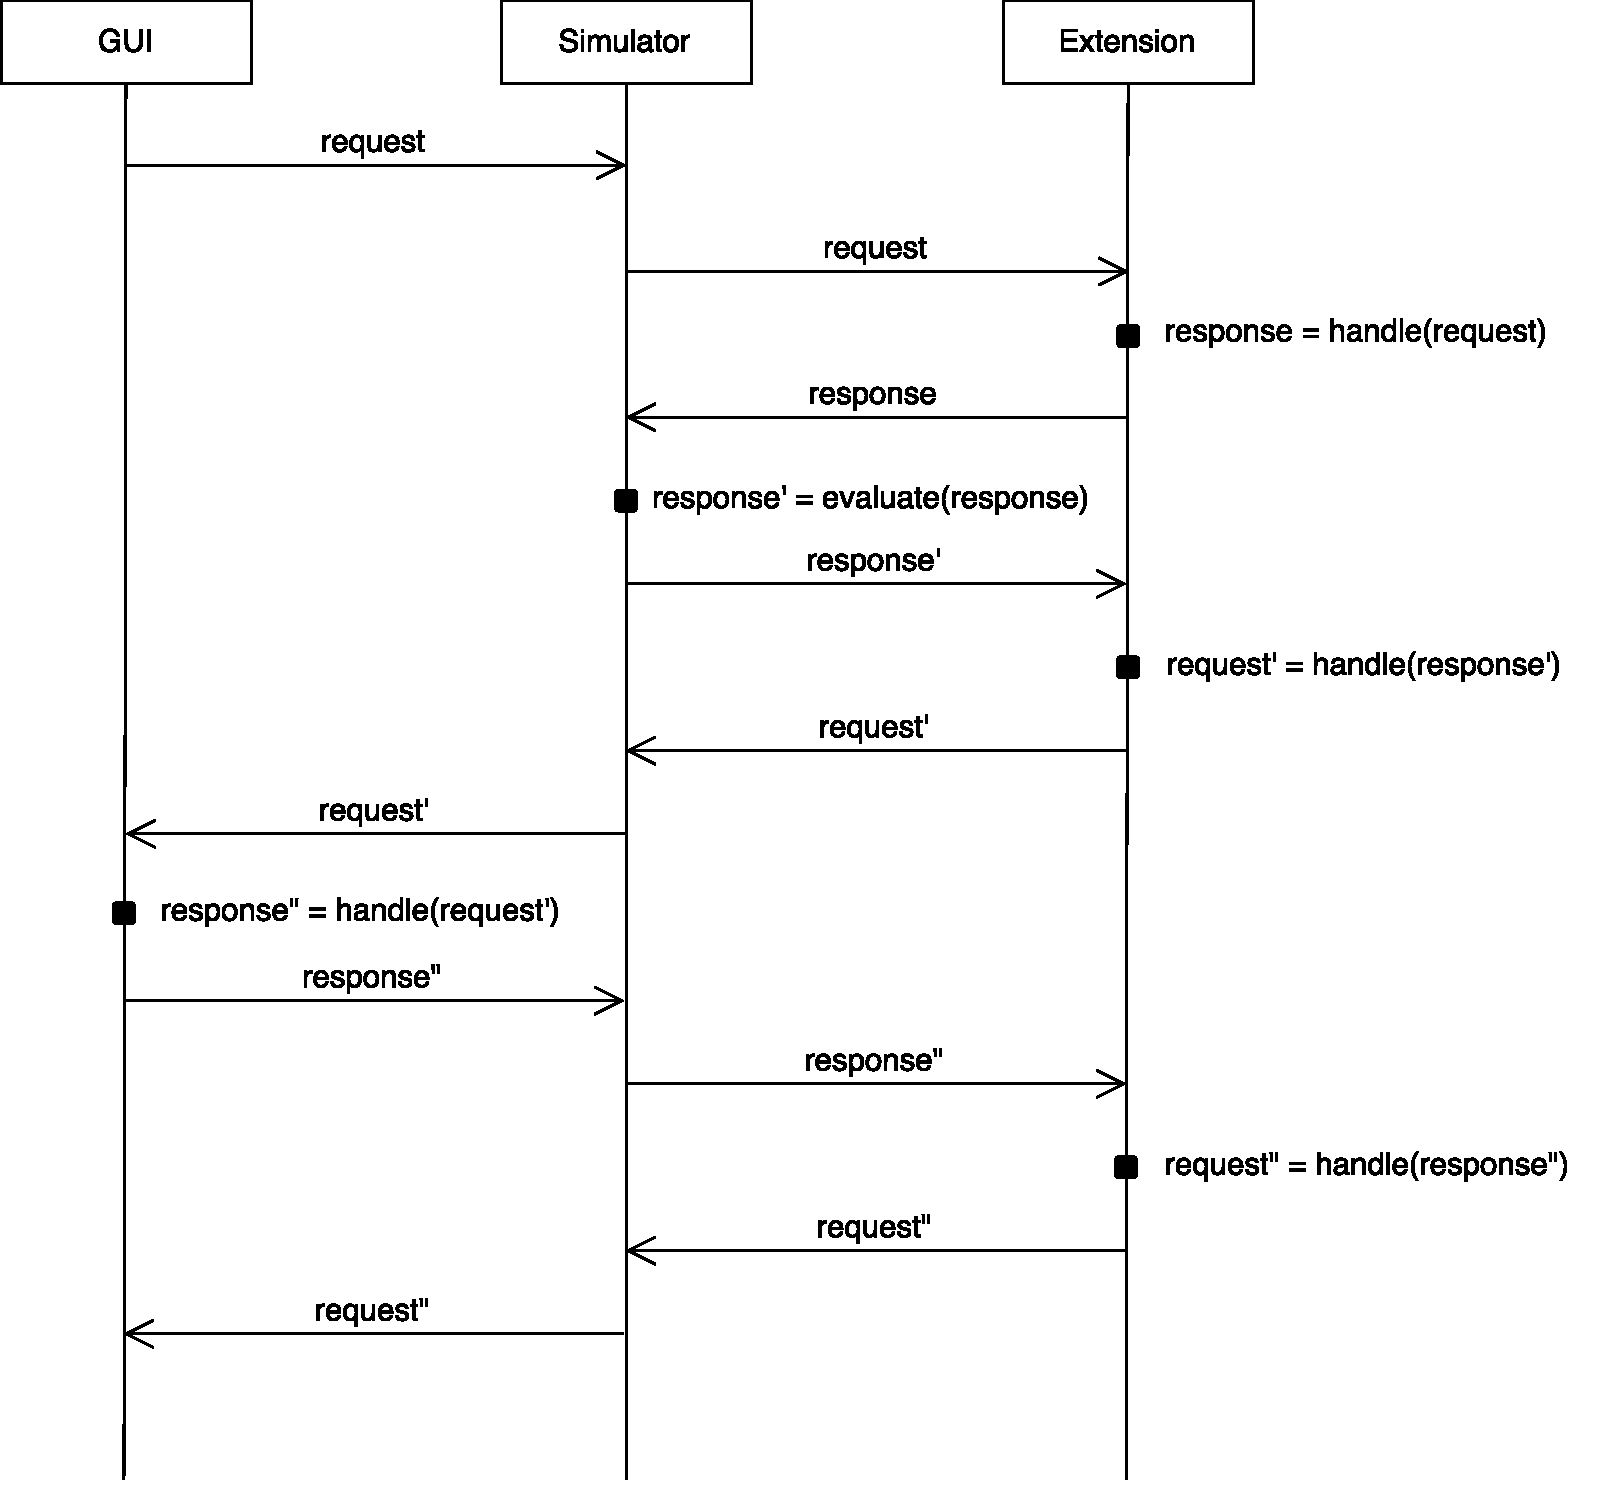
\includegraphics[scale = 0.40]{DBN_Impl_Extension_Communication_Pattern.pdf}
	\caption{Communication Pattern of CPN Tools extensions}
	\label{fig:DBN_Impl_Extension_Communication_Pattern}
\end{figure}
}}
\subparagraph*{\textnormal{In Figure \ref{fig:DBN_Impl_Extension_Communication_Pattern}, when a subscribed event occurs, the messages are passed from the GUI to the simulator over the channel. We call such messages as \textit{requests}. The extension takes appropriate response on the request and passes the response to the simulator. Simulator checks whether the response could be safely incorporated by the GUI, i.e., the response should not bring CPN Tools to an inconsistent state and returns its evaluation to the extension. Once the evaluation is received, the extension handles the evaluated response and makes a request to update the GUI. Once the request is incorporated/rejected by GUI, the corresponding response is sent to the extension. Extension handles the received response and gives the control back to the GUI.}}

\subparagraph*{\textnormal{Let us see an example of populating view places using the communication pattern presented in Figure \ref{fig:DBN_Impl_Extension_Communication_Pattern}. When we declare a view place, the extension determines the declaration by scanning the net. In this case, the \textit{request} is passed from the GUI to the extension via simulator. The extension \textit{handles} the \textit{request} and takes appropriate \textit{response} by fetching the marking (for the view place) from the database. However, at this stage, the extension does not know if the markings are compatible with the colour-set of the view place. In order to verify if the marking is compatible with the colour set of the view place, the \textit{response} is passed to the simulator. The simulator evaluates (verification of the marking) the \textit{response} and provides its decision (\textit{response\textquotesingle}) to the extension whether the marking is compatible with the colour set of the view place. Upon receiving the evaluation, extension handles it and in case the marking is compatible, it creates a new request (\textit{request\textquotesingle}) to update the marking of the view place and passes on to the GUI via simulator. On receiving the new request (\textit{request\textquotesingle}), the GUI updates the marking of the view place. After incorporating the request (by changing the marking of view place), the GUI sends a response (\textit{response\textquotedbl}) to the extension whether the request (\textit{request\textquotesingle}) was successfully incorporated or not. Upon receiving the response (\textit{response\textquotedbl}), the extension handles it and gives back the control to the GUI.}}

\subparagraph*{\textnormal{Similarly, on subscription basis, the extension receives the notification once we write any declaration, e.g., colour-set, variables etc., in CPN Tools. The extension also receives the notification when a model is loaded or saved in CPN Tools. Simulation related messages, e.g., firing of transitions, enabledness of transitions, markings of the places etc. are also subscribed. This extension is registered to CPN Tools extension server, used to boot all the registered extensions, and loaded as soon as CPN Tools is started.}}

\subsubsection*{Poll Server}
\subparagraph*{\textnormal{\textit{Poll Server} is a JAVA process which comprises of JAVA functions intended to execute actions attached to the transitions and facilitate data acquisition. The \textit{Poll Server} is connected to CPN Tools with JAVA/CPN and also connected to the database (Postgres SQL) through JDBC. The JAVA functions written in \textit{Poll Server} for facilitating data acquisition and executing actions can be called in an indirect way from CPN Tools using Comms/CPN APIs. We encapsulate the name of the JAVA functions (contained in \textit{Poll Server}) along with its parameters in a formatted string and send it through Comms/CPN. When the formatted string is received, it is parsed and the corresponding function with corresponding parameters is called. These functions can possibly have many internal APIs which can be called by passing the function API as a parameter. Currently, we provide three functions in the \textit{Poll Server} which are:
\begin{enumerate}
\item \textit{getRandom} - takes two parameters in order: \textit{funcAPI} and \textit{length}. The function API (\textit{funcAPI}) can be either \textit{randomInt}, \textit{randomString} or \textit{randomTime}. Based on the function API, data logic layer decides which function should be called and returns the result of the specified length. Currently, the function API \textit{randomTime} returns a random time in $\langle hh:mm:ss \rangle$ format which is compatible with SQL.
\item \textit{getFromDB} - takes four parameters in order: \textit{funcAPI}, \textit{tableName}, \textit{columnName} and \textit{length}. Currently, the supported function API (\textit{funcAPI}) is \textit{genUniqueID}, which generates a random unique identifier of given length for the specified \textit{tableName} and \textit{columnName}.
\item \textit{exQuery} - takes one parameter: \textit{query}. This function executes the given query.
\end{enumerate}
}}

\section{DB-nets example}
\label{sec:DBN_Impl_DBN_example}
\paragraph*{\textnormal{In this section, we will discuss the taxi booking example discussed in the previous chapter. First, we discuss our database schema and then we take the example of the CPN drawn for the taxi booking example in the previous chapters. We transform the CPN into a DB-net while explaining modelling guidelines for action transitions and view places.}}

\subparagraph*{\textnormal{We start with modelling our database schema in PostgresSQL. We name our database schema as \bdsq{taxi\_booking} (see Figure \ref{fig:DBN_Impl_Persistence_Layer}) which contains tables and constraints. The table \textit{session} contains the unique session ids generated for each booking session. The table \textit{taxi}, \textit{phone} and \textit{pickup\_data} contains information regarding taxi, customer's phone details and pickup details. \textit{booking} table stores data related to the final booking. As indicated in Figure \ref{fig:DBN_Impl_Persistence_Layer}, the database schema also contains primary key and foreign key constraints\footnote{primary keys and foreign are indicated in the schema using underlines and arrows respectively.}.}}

\begin{figure}[!htbp]
	\centering
	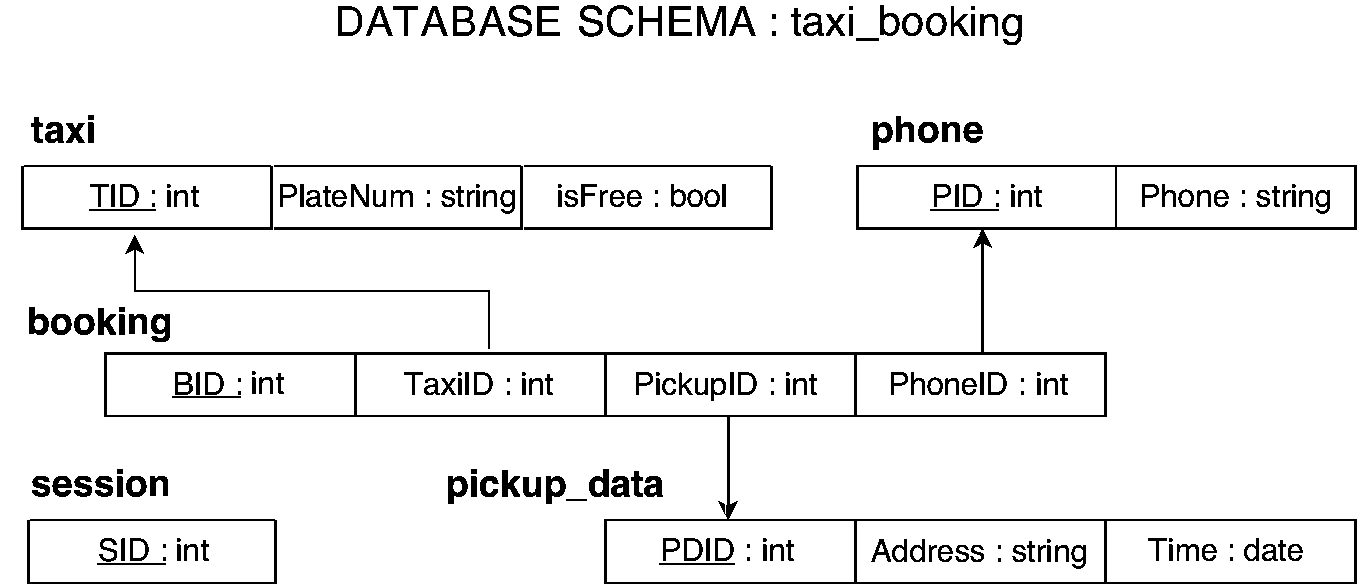
\includegraphics[scale = 0.45]{DBN_Impl_Persistence_Layer.pdf}
	\caption{Database Schema for taxi booking example}
	\label{fig:DBN_Impl_Persistence_Layer}
\end{figure}

\subparagraph*{\textnormal{In Figure \ref{fig:DBN_Impl_CPN_Taxi_Booking}, we present the CPN model of the taxi booking example presented in previous chapters. In this example, we transform the $\mathit{Free\ Taxi}$ place into a view place which would represent taxis available for booking. We also transform $\mathit{Create\ Booking}$ transition into an action transition, which will make the selected taxi unavailable for further booking. We connect $\mathit{Free\ Taxi}$ view place and $\mathit{Create\ Booking}$ transition with a read arc\footnote{The read arc is modelled as a doubled headed arc in CPN Tools.} (see Figure \ref{fig:DBN_Impl_Control_Layer}).}}

\begin{figure}[!htbp]
	\centering
	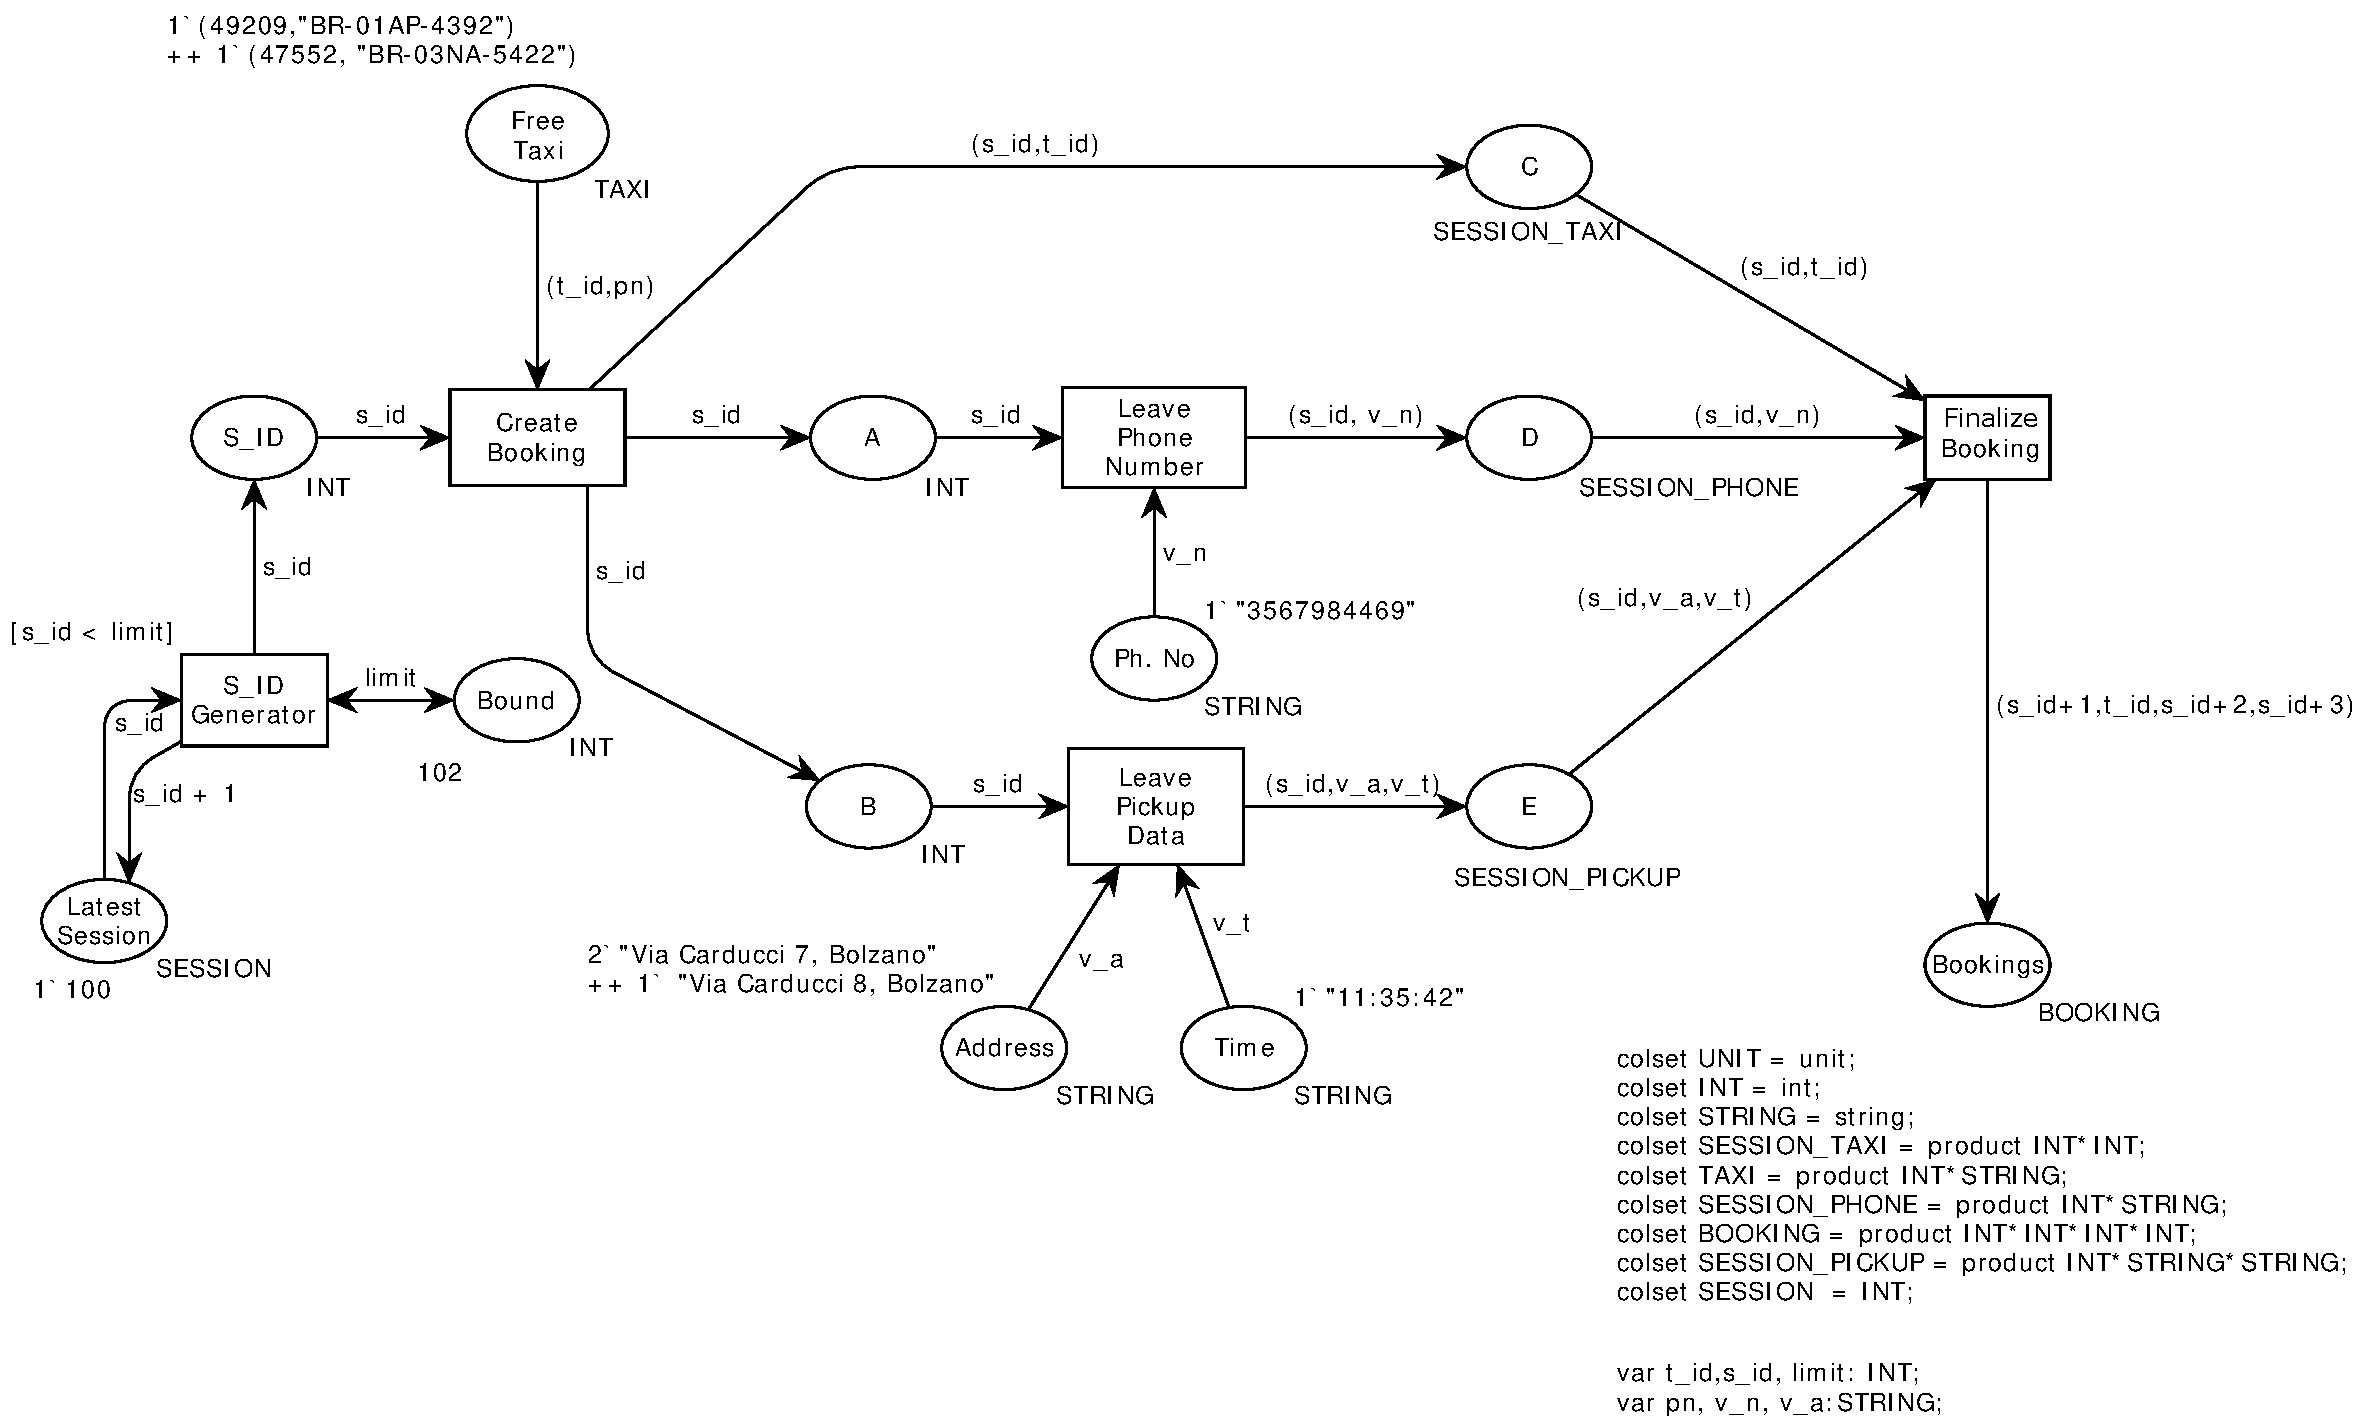
\includegraphics[scale = 0.35]{DBN_Impl_CPN_Taxi_Booking.pdf}
	\caption{CPN model for taxi booking example}
	\label{fig:DBN_Impl_CPN_Taxi_Booking}
\end{figure}

\begin{figure}[!htbp]
	\centering
	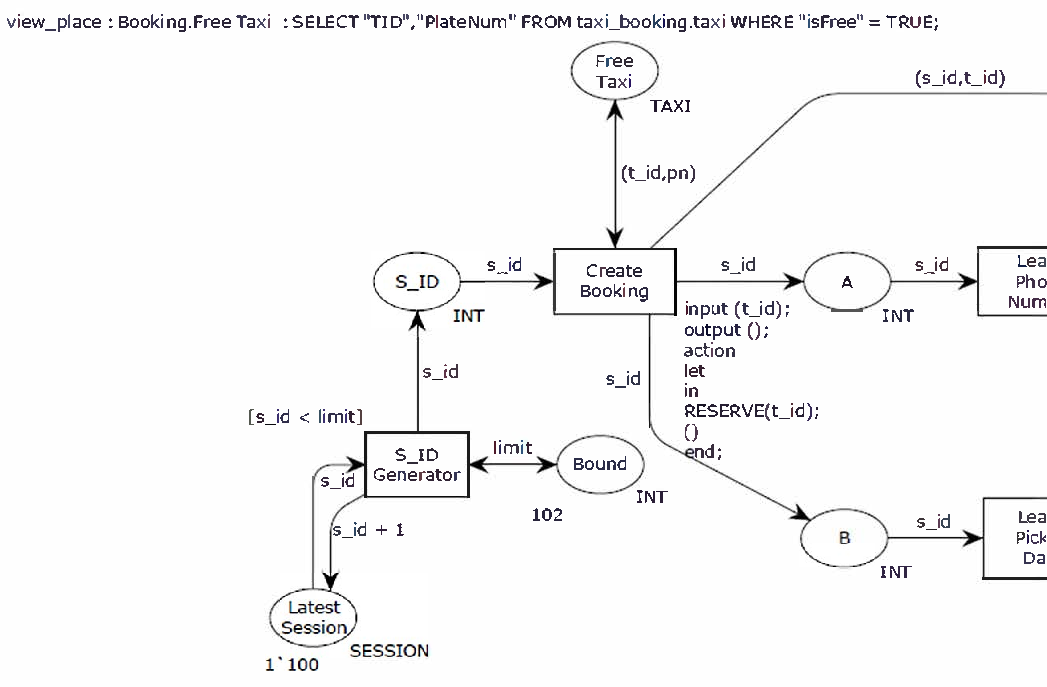
\includegraphics[scale = 0.60]{DBN_Impl_Control_Layer.pdf}
	\caption{View Place, Action Transition and Read Arcs representation}
	\label{fig:DBN_Impl_Control_Layer}
\end{figure}

\subparagraph*{\textnormal{In Figure \ref{fig:DBN_Impl_Control_Layer}, following the syntax, we define the view place using the \bsq{Text} tool and write the query attached to the view place as:}}

\subparagraph*{}
\begin{lstlisting}[showstringspaces=false, language = ML, caption = View place definition: $\mathit{Free\ Taxi}$, captionpos=b]
view_place : Booking.Free Taxi : SELECT "TID","PlateNum" FROM taxi_booking.taxi WHERE "isFree" = TRUE;
\end{lstlisting}

\subparagraph*{\textnormal{In Figure \ref{fig:DBN_Impl_Control_Layer}, the code segment of the \textit{Create Booking} transition is written as:}}

\subparagraph*{}

\begin{lstlisting}[showstringspaces=false, language = ML, caption = Code Segment: \textit{Create Booking} transition, captionpos=b, label = lst:DBN_Impl_Create_Booking_code_segment, numbers=left,
stepnumber=1]
input(t_id);
output();
action
let
in
RESERVE(t_id);
()
end;
\end{lstlisting}

\subparagraph*{\textnormal{In the code segment above, the \textit{Create Booking} transition takes a taxi id in the input part and performs an \textit{RESERVE} action related with the taxi id in the action part. The \textit{RESERVE} action is an update operation, which makes the taxi unavailable for further booking. These actions are just ML functions which we will discuss later in the chapter.}}

%\subparagraph*{\textnormal{Note that $\mathit{Create\ Booking}$ transition has a $\mathit{RESERVE}$ action attached to it. Using code segment of the transition, we could write the action part of the transition. The $\mathit{RESERVE}$ action is defined as an ML function\footnote{These ML functions are written in the declaration column in CPN Tools}:}}
%
%\subparagraph*{}
%
%\begin{lstlisting}[showstringspaces=false, language = ML, caption = RESERVE action, captionpos=b, label = lst:DBN_Impl_RESERVE_action_query]
%fun RESERVE(t_id) = exQuery("UPDATE taxi_booking.taxi SET \"isFree\" = FALSE WHERE \"TID\" ="^ Int.toString t_id^";");
%\end{lstlisting}
%
%\subparagraph*{\textnormal{\textit{exQuery} is an ML function which takes the query\footnote{In the query, (see Listing \ref{lst:DBN_Impl_RESERVE_action_query}), the {\textbackslash \textquotedbl} symbol is used in ML to represent double quotes in string where as $\string^$ symbol is used to concatenate two strings.} as a parameter and passes it to Comms/CPN for execution.}}

\subparagraph*{\textnormal{$\mathit{Leave\ Phone\ Number}$ and $\mathit{Leave\ Pickup\ Data}$ transitions are also transformed into action transition. These transitions carry fresh variables which are used for acquiring data from the environment. We remove the places $\mathit{Ph. No}$, $\mathit{Address}$ and $\mathit{Time}$ (see Figure \ref{fig:DBN_Impl_CPN_Taxi_Booking}), and acquire data in the code segment of \textit{Leave Phone Number} and $\mathit{Leave\ Pickup\ Data}$ transitions (see Figure \ref{fig:DBN_Impl_Data_Acquisition}).}}

\begin{figure}[!htbp]
	\centering
	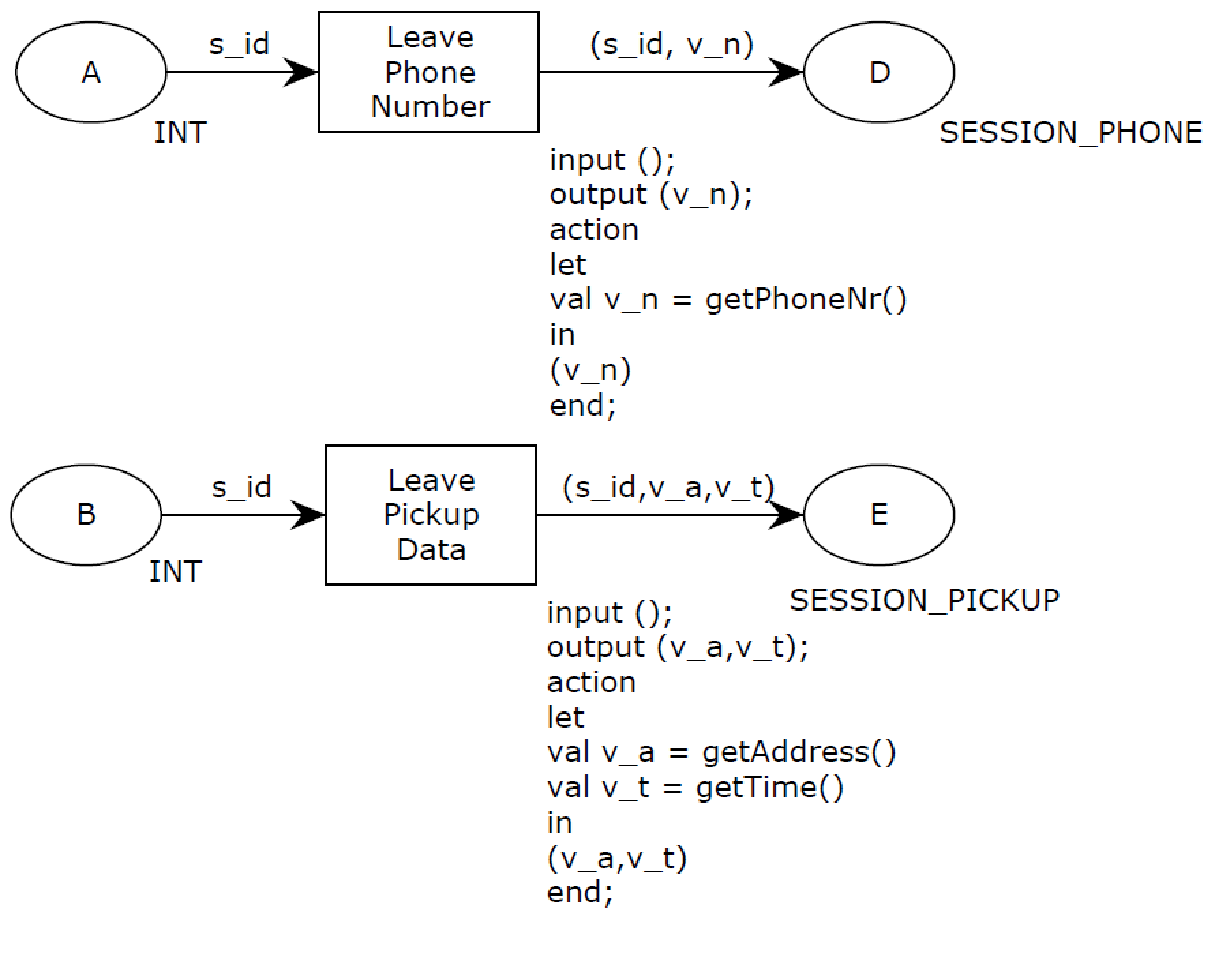
\includegraphics[scale = 0.35]{DBN_Impl_Data_Acquisition.pdf}
	\caption{Action transitions: Leave Phone Number and Leave Pickup Data}
	\label{fig:DBN_Impl_Data_Acquisition}
\end{figure}

\subparagraph*{\textnormal{The code segment of \textit{Leave Phone Number} transition is shown in Listing \ref{lst:DBN_Impl_code_segment_leave_ph_number} and the one of $\mathit{Leave\ Pickup\ Address}$ is shown in Listing \ref{lst:DBN_Impl_code_segment_leave_picup_data}. In the \textit{Leave Phone Number} transition, the fresh variable $\mathit{v\_n}$ acquires the phone number from the ML function $\mathit{getPhoneNr}$. Similarly, in the $\mathit{Leave\ Pickup\ Data}$ transition, the variables $\mathit{v\_a}$ and $\mathit{v\_t}$ acquire pickup address and time from the ML functions $\mathit{getAddress}$ and $\mathit{getTime}$ respectively. Hence, instead of providing the data before hand (as marking on places $\mathit{Ph. No}$, $\mathit{Address}$ and $\mathit{Time}$), we acquire data dynamically from the external environment.}}
\subparagraph*{}
\begin{lstlisting}[showstringspaces=false, language = ML, caption = Code segment of transition: $\mathit{LEAVE\ PHONE\ NUMBER}$, captionpos=b, label = lst:DBN_Impl_code_segment_leave_ph_number, numbers=left,
stepnumber=1]
input()
output(v_n)
let
val v_n = getPhoneNr()
in
(v_n)
end;
\end{lstlisting}

\subparagraph*{}
\begin{lstlisting}[showstringspaces=false, language = ML, caption = Code segment of transition: $\mathit{LEAVE\ PICKUP\ DATA}$, captionpos=b, label = lst:DBN_Impl_code_segment_leave_picup_data, numbers=left,
stepnumber=1]
input();
output(v_a,v_t);
action
let
val v_a = getAddress()
val v_t = getTime()
in
(v_a,v_t)
end;
\end{lstlisting}

\subparagraph*{\textnormal{In the CPN model (Figure \ref{fig:DBN_Impl_CPN_Taxi_Booking}), the transition $\mathit{S\_ID\ Generator}$ generates two session id in the range [100,101], however, it is not guaranteed that these generated session ids are unique to our relational schema \textit{session}. In order to make it unique to the session table, we transform this transition into an action transition, and using a fresh variable $\mathit{s\_id}$ we acquire a unique identifier by consulting the \textit{session} table. The transformation for the part of session id generation is shown in Figure \ref{fig:DBN_Impl_SID_Generator}. Note that, the number of session ids which can be generated is no more bounded. One could create the upper bound by introducing the $\mathit{Bound}$ place and the guard over the transition.}}

\begin{figure}[!htbp]
	\centering
	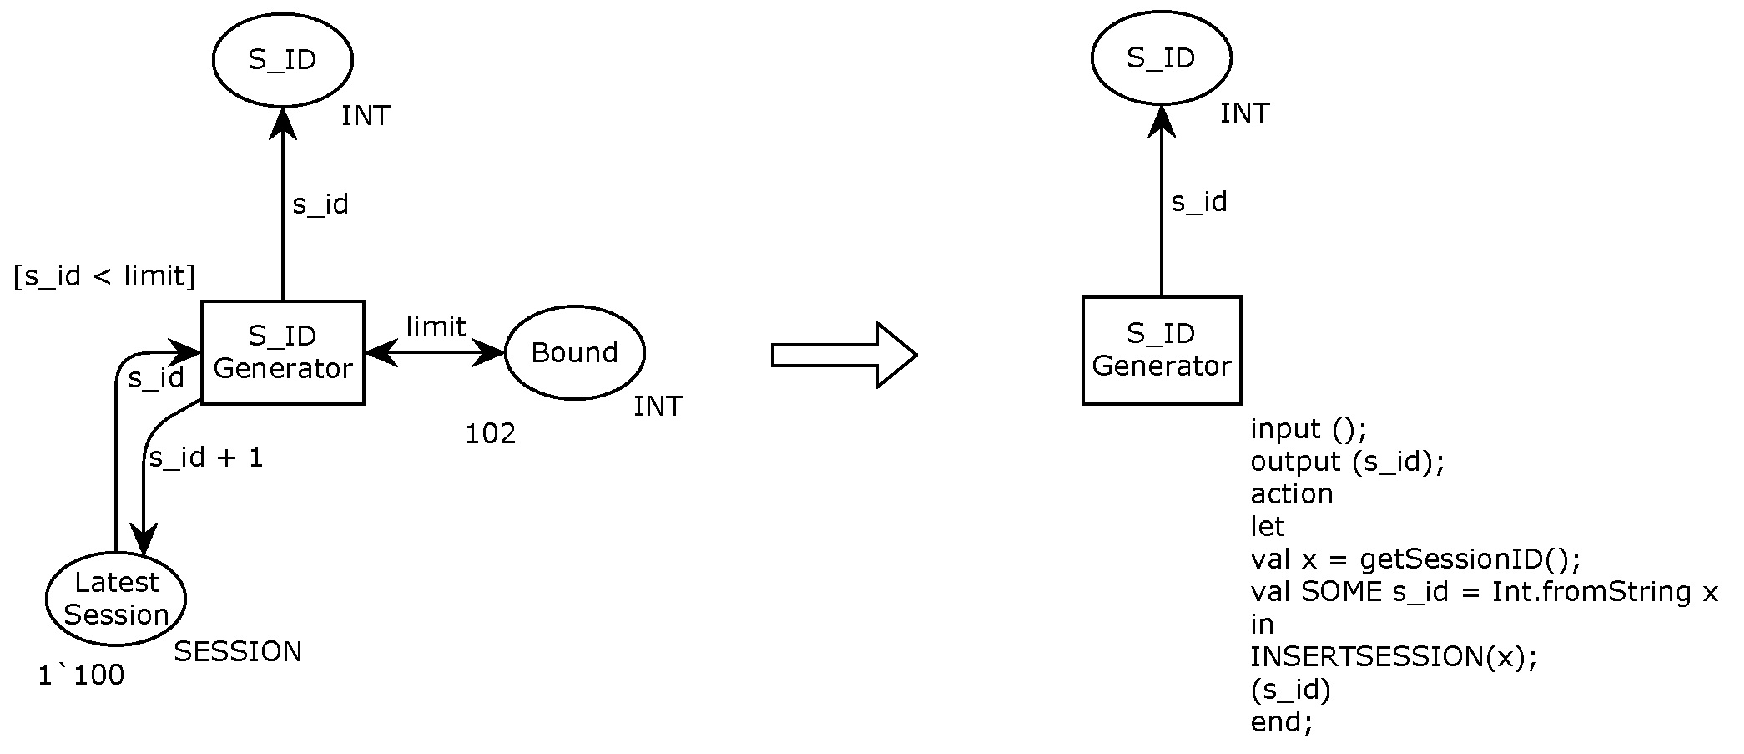
\includegraphics[scale = 0.35]{DBN_Impl_SID_Generator.pdf}
	\caption{S\_ID Generator}
	\label{fig:DBN_Impl_SID_Generator}
\end{figure}

\subparagraph*{\textnormal{The code segment of the transition $\mathit{S\_ID\ Genearator}$ is shown in Listing \ref{lst:DBN_Impl_code_segment_sid_gen}. At line 5, the ML function $\mathit{getSessionID}$ internally use Comms/CPN API and returns a unique session identifier in string format. Since the place $\mathit{S\_ID}$ has the colour-set $\mathit{INT}$, the identifier is converted to the $\mathit{INT}$ type (line number 6). In order to restrict the system from generating the same session id again, the generated session id is inserted in the \textit{session} table (line number 8) using an ML function $\mathit{INSERTSESSION}$ which internally use Comms/CPN APIs. In the end, the unique session id is generated and can be used for booking purpose.}}

\subparagraph*{}
\begin{lstlisting}[showstringspaces=false, language = ML, caption = code segment of transition : $\mathit{S\_ID\ Generator}$, captionpos=b, label = lst:DBN_Impl_code_segment_sid_gen, numbers=left,
stepnumber=1]
input();
output(s_id);
action
let
val x = getSessionID();
val SOME s_id = Int.fromString x 
in
INSERTSESSION(x);
(s_id)
end;
\end{lstlisting}

\subparagraph*{\textnormal{Similarly, we could transform $\mathit{Finalize\ Booking}$ transition as shown in Figure \ref{fig:DBN_Impl_Finalize_Booking} where $\mathit{b\_id}$, $\mathit{pd\_id}$ and $\mathit{ph\_id}$ are of \textit{INT} data type and represent booking id, pickup id and phone id respectively. The booking id, pickup id and the phone id are generated by consulting the respective tables and sequentially inserted. The code segment of $\mathit{Finalize\ Booking}$ transition is given in Listing \ref{lst:DBN_Impl_code_segment_add_booking} where $\mathit{getBookingID}$, $\mathit{getPickupID}$ and $\mathit{getPhoneID}$ are ML functions which fetch a unique id for the respective tables. $\mathit{INSERTPHONE}$, $\mathit{INSERTPICKUP}$ and $\mathit{ADDBOOKING}$ functions insert records in the corresponding relational database. Note that the order of insertion of these records matters due to the presence of the foreign key constraints. For example, the foreign key between $\mathit{booking}$ table and $\mathit{pickup\_data}$ table, allows insertion of a tuple, in $\mathit{booking}$ table, containing pickup id only when the corresponding pickup id is present in the $\mathit{pickup\_data}$ table. Similarly, one cannot remove a tuple from the $\mathit{pickup\_data}$ table if the corresponding $\mathit{pickup_id}$ is referenced in the $\mathit{booking}$ table.}}

\begin{figure}[!htbp]
	\centering
	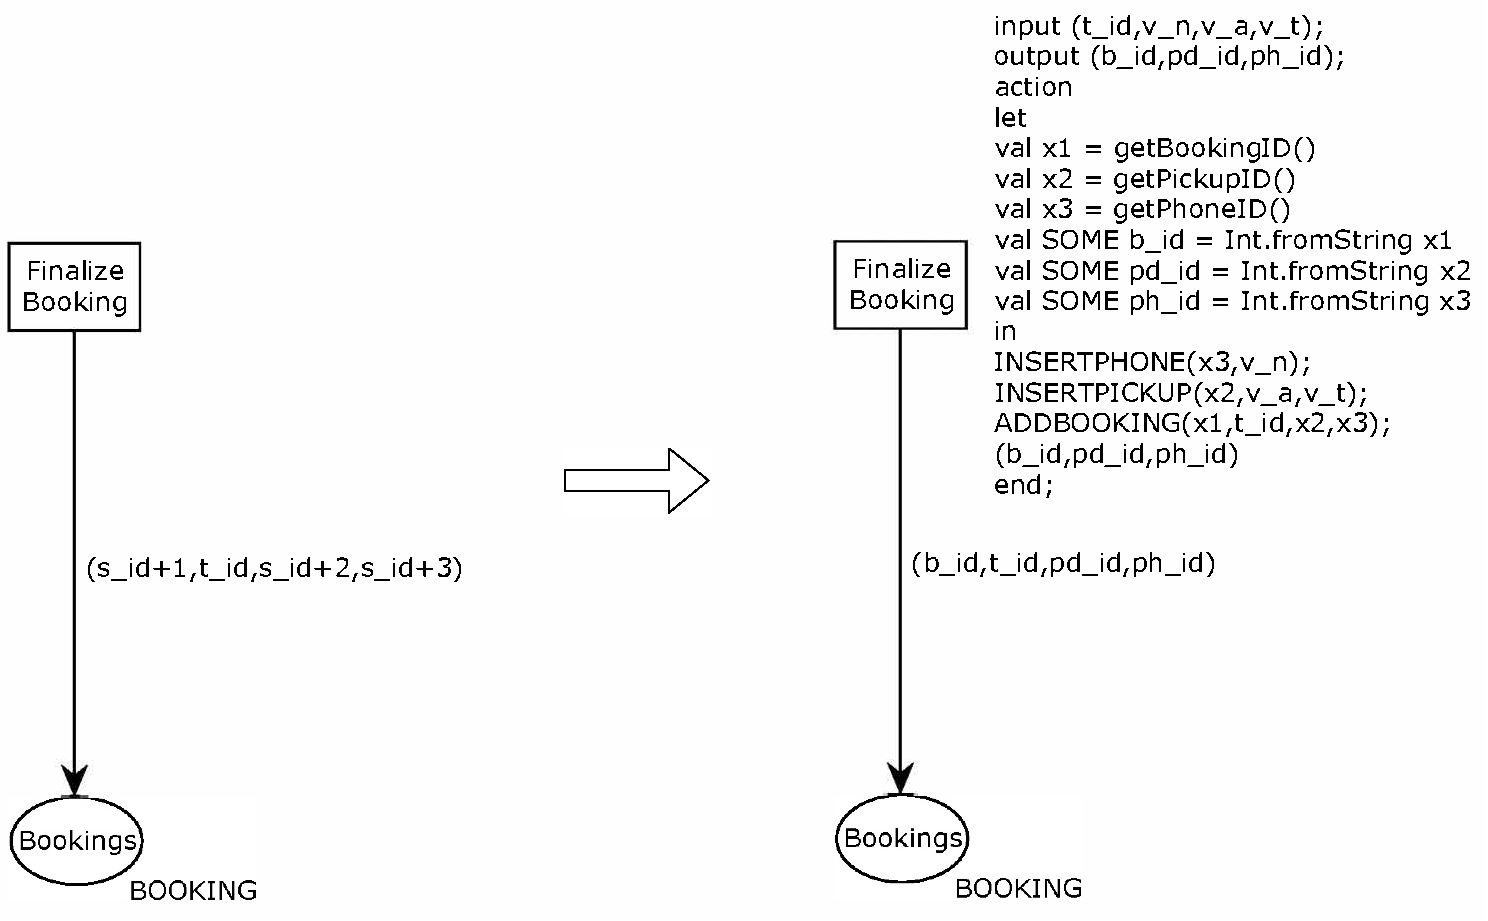
\includegraphics[scale = 0.35]{DBN_Impl_Finalize_Booking.pdf}
	\caption{$\mathit{Add\ Booking}$ transition}
	\label{fig:DBN_Impl_Finalize_Booking}
\end{figure}

\subparagraph*{}
\begin{lstlisting}[showstringspaces=false, language = ML, caption = code segment of transition : $\mathit{Finalize\ Booking}$, captionpos=b, label = lst:DBN_Impl_code_segment_add_booking, numbers=left,
stepnumber=1]
input(t_id,v_n,v_a,v_t);
output(b_id,pd_id,ph_id);
action
let
val x1 = getBookingID()
val x2 = getPickupID()
val x3 = getPhoneID()
val SOME b_id = Int.fromString x1
val SOME pd_id = Int.fromString x2
val SOME ph_id = Int.fromString x3
in
INSERTPHONE(x3,v_n);
INSERTPICKUP(x2,v_a,v_t);
ADDBOOKING(x1,t_id,x2,x3);
(b_id,pd_id,ph_id)
end;
\end{lstlisting}

\subparagraph*{\textnormal{We provide three ML functions which internally call Comms/CPN APIs and are able to communicate using the unique connection name. Users are encouraged to use these ML functions in order to interact with the database. One can also write their own ML functions and use them in a similar way. For example, one of the three ML function which we provide, $\mathit{exQuery}$ can be written as:}}

\subparagraph*{}
\begin{lstlisting}[showstringspaces=false, language = ML, caption = exQuery function, captionpos=b, label = lst:DBN_Impl_exQuery]
fun exQuery(connectionName, query) = ConnManagementLayer.send(connectionName, "exQuery"^"?"^query, stringEncode);
\end{lstlisting}

\subparagraph*{\textnormal{In the above function, the $\string^$ symbol is used to concatenate two strings in ML. The \bdsq{?} sign separates part of the string and is used to provide a marker to the parser in the \textit{Poll Server} to identify different parts of the string received from Comms/CPN. The $\mathit{exQuery}$ function takes the connection name as the first parameter, followed by the function name to be called\footnote{Here \bdsq{exQuery} is the function name in the \textit{Poll Server}.} in the \textit{Poll Server} and the query to be executed.}}

\subparagraph*{\textnormal{Let us consider an example for executing a query using the $\mathit{exQuery}$ function. The $\mathit{RESERVE}$ action mentioned in the code segment of $\mathit{Create\ Booking}$ (see Listing \ref{lst:DBN_Impl_Create_Booking_code_segment}) transition can be written as an ML function:}}

\subparagraph*{title}
\begin{lstlisting}[showstringspaces=false, language = ML, caption = RESERVE action, captionpos=b, label = lst:DBN_Impl_RESERVE_action_query]
fun RESERVE(t_id) = exQuery("Taxi_Connection","UPDATE taxi_booking.taxi SET \"isFree\" = FALSE WHERE \"TID\" ="^ Int.toString t_id^";");
\end{lstlisting}

\subparagraph*{\textnormal{In Listing \ref{lst:DBN_Impl_RESERVE_action_query} \footnote{In ML, the {\textbackslash \textquotedbl} symbol is used to represent double quotes in strings.}, we specify the connection name as $\mathit{Taxi\_Connection}$, followed by the query to be executed. As the first parameter, we specify the connection name as $\mathit{Taxi\_Connection}$, which will be used throughout our example. The query (in the \textit{RESERVE} function) updates the $\mathit{taxi}$ table and makes the selected taxi unavailable for booking. For example, for $\mathit{t\_id = 47552}$, the query passed would be :}}

\subparagraph*{}
\begin{lstlisting}[showstringspaces=false, language = SQL, caption = RESERVE action: query example, captionpos=b, label = lst:DBN_Impl_RESERVE_action_query_ex]
UPDATE taxi_booking.taxi SET "isFree" = FALSE WHERE "TID" = 47552;
\end{lstlisting}

\subparagraph*{\textnormal{The other two functions which we provide are $\mathit{getFromDB}$ and $\mathit{getRandom}$ which can be written as:}}

\subparagraph*{}
\begin{lstlisting}[showstringspaces=false, language = ML, caption = \textit{getRandom} and \textit{getFromDB} function, captionpos=b, label = lst:DBN_Impl_provided_APIs, numbers=left,
stepnumber=1]
fun getFromDB(connectionName, funcAPI, t_name, c_name, length) = (ConnManagementLayer.send(connectionName, "getFromDB"^"?"^t_name^"?"^c_name^"?"^funcAPI^"?"^length, stringEncode); ConnManagementLayer.receive(connectionName, stringDecode));
fun getRandom(connectionName, funcAPI, length) = (ConnManagementLayer.send(connectionName, "getRandom"^"?"^funcAPI^"?"^length, stringEncode); ConnManagementLayer.receive(connectionName, stringDecode));
\end{lstlisting}

\subparagraph*{\textnormal{In a similar manner as \textit{exQuery}, while sending data, \textit{getFromDB} and \textit{getRandom} encapsulate the function name which needs to be called by the \textit{Poll Server}. Following the function name, the function APIs are specified, i.e., the different flavours of the function which are offered. For $\mathit{getFromDB}$ function, currently, the supported API is only \textit{genUniqueID}. For \textit{getRandom} function, the supported APIs are \textit{getRandomInt}, \textit{getRandomString} and \textit{getRandomTime}. We use these functions (mentioned in Listing \ref{lst:DBN_Impl_provided_APIs}) for data acquisition.}}

\subparagraph*{\textnormal{In order to complete the modelling phase in CPN Tools, we have to explicitly define the ML functions called in the code segment of each transition\footnote{We assume that the user is familiar with the declaration of colour-set and variables.}(if any). The function $\mathit{getSessionID}$ and $\mathit{INSERTSESSION}$, mentioned in the code segment of $\mathit{S\_ID\ Generator}$ transition, can be defined as:}}

\subparagraph*{}
\begin{lstlisting}[showstringspaces=false, language = ML, caption = Functions for generating and inserting session ID, captionpos=b, label = lst:DBN_Impl_functions_SID_Gen,numbers=left,
stepnumber=1]
fun getSessionID() = getFromDB("Taxi_Connection","genUniqueID","taxi_booking.session","\"SID\"","6");
fun INSERTSESSION(s_id) = exQuery("Taxi_Connection","INSERT INTO taxi_booking.session VALUES ("^ s_id ^ ");" );
\end{lstlisting}

\subparagraph*{\textnormal{In the function $\mathit{getSessionID}$, we pass the first parameter as the connection name, the second parameter is the function API which needs to be called. $\mathit{taxi\_booking.session}$ is the session table in the $\mathit{taxi\_booking}$ schema which is passed as the third parameter, followed by the column name for which the unique id is to be generated, and finally, we pass the length of the desired identifier. In our case, we generate a 6 digit unique random identifier. The definition of the function $\mathit{INSERTSESSION}$ is similar to the \textit{RESERVE} function as it internally uses the $\mathit{exQuery}$ function. However, the query in the $\mathit{INSERTSESSION}$ function performs insertion in the $\mathit{session}$ table.}}

\subparagraph*{\textnormal{Similarly, one could write ML functions in the code segment of \textit{Finalize Booking} transition. The ML functions $\mathit{getBookingID}$, $\mathit{getPickupID}$ and $\mathit{getPhoneID}$ could be modelled similar to the function $\mathit{getSessionID}$, and \textit{INSERTPHONE}, \textit{INSERTPICKUP} and \textit{ADDBOOKING} could be modelled similar to $\mathit{getSessionID}$ functions. Transitions such as \textit{Leave Phone Number} and \textit{Leave Pickup Data} use ML functions \textit{getPhoneNr}, \textit{getAddress} and \textit{getTime} function to acquire a random phone number, random address and random time. These functions could be written as:}}

\subparagraph*{}
\begin{lstlisting}[showstringspaces=false, language = ML, caption = {Functions for acquiring random phone number, random address and random time}, captionpos=b, label = lst:DBN_Impl_Leave_Phone,numbers=left,
stepnumber=1]
fun getPhoneNr()=getRandom("Taxi_Connection","randomInt","10");
fun getAddress()=getRandom("Taxi_Connection","randomString","20");
fun getTime()=getRandom("Taxi_Connection","randomTime","6");
\end{lstlisting}

\subparagraph*{\textnormal{As mentioned earlier, the \textit{getRandom} function provides three different inputs based on predefined modes, \textit{randomInt}, \textit{randomString} and \textit{randomTime}. For example, the function \textit{getPhoneNr} returns a phone number (of string type) of length 10. Similarly, \textit{getAddress} function returns a random address which is a combination of 20 characters and \textit{getTime} function returns a time in $\langle hh:mm:ss \rangle$ format\footnote{This format is compatible with SQL. The length in the $\mathit{getTime}$ function is fixed right now.}.}}

\subparagraph*{\textnormal{In order to connect to a TCP/IP port, we also specify functions namely \textit{connectDB} and \textit{disconnectDB} which internally use Comms/CPN APIs and connect to the specified TCP/IP port. These functions are declared as:}}

\subparagraph*{}
\begin{lstlisting}[showstringspaces=false, language = ML, caption = {Functions for acquiring random phone number, random address and random time}, captionpos=b, label = lst:DBN_Impl_Connect_Disconnect,numbers=left,
stepnumber=1]
fun connectDB(connectionName, port) = ConnManagementLayer.acceptConnection(connectionName, port);
fun disconnectDB(connectionName) = ConnManagementLayer.closeConnection(connectionName);
\end{lstlisting}
\subparagraph*{\textnormal{In order to call \textit{connectDB} and \textit{disconnectDB} functions, we write our code in the net using the \bsq{Text} Tool. For example, we could use \bdsq{Taxi\_Connection} as the connection name and 9000 as the port number in the connection parameters.}}
\begin{verbatim}
connectDB("Taxi_Connection", 9000)
disconnectDB("Taxi_Connection")
\end{verbatim}

\subparagraph*{\textnormal{We need to run this code using the \bsq{ML} tool which evaluates a text as an ML code. Note that the above two mentioned code should be written in separate text boxes.}}

\subparagraph*{\textnormal{Till now, we have modelled our database schema (see Figure \ref{fig:DBN_Impl_Persistence_Layer}) in Postgres SQL and our DB-net (see Figure \ref{fig:DBN_Impl_executable_model}) in CPN Tools. The next step is to establish the connection for the information flow between these two components. As stated earlier, the extension starts when CPN Tools is started and listens to all the subscribed events. In order to facilitate connection with the database, our extension provides an interface (see Figure \ref{fig:DBN_Impl_Extension_Dialog}) where the user has to provide parameters for the database connection. Once the user sets up the connection, the extension scans the DB-net model, identifies the view places and updates the marking of the view places.}}

\begin{figure}[!htbp]
	\centering
	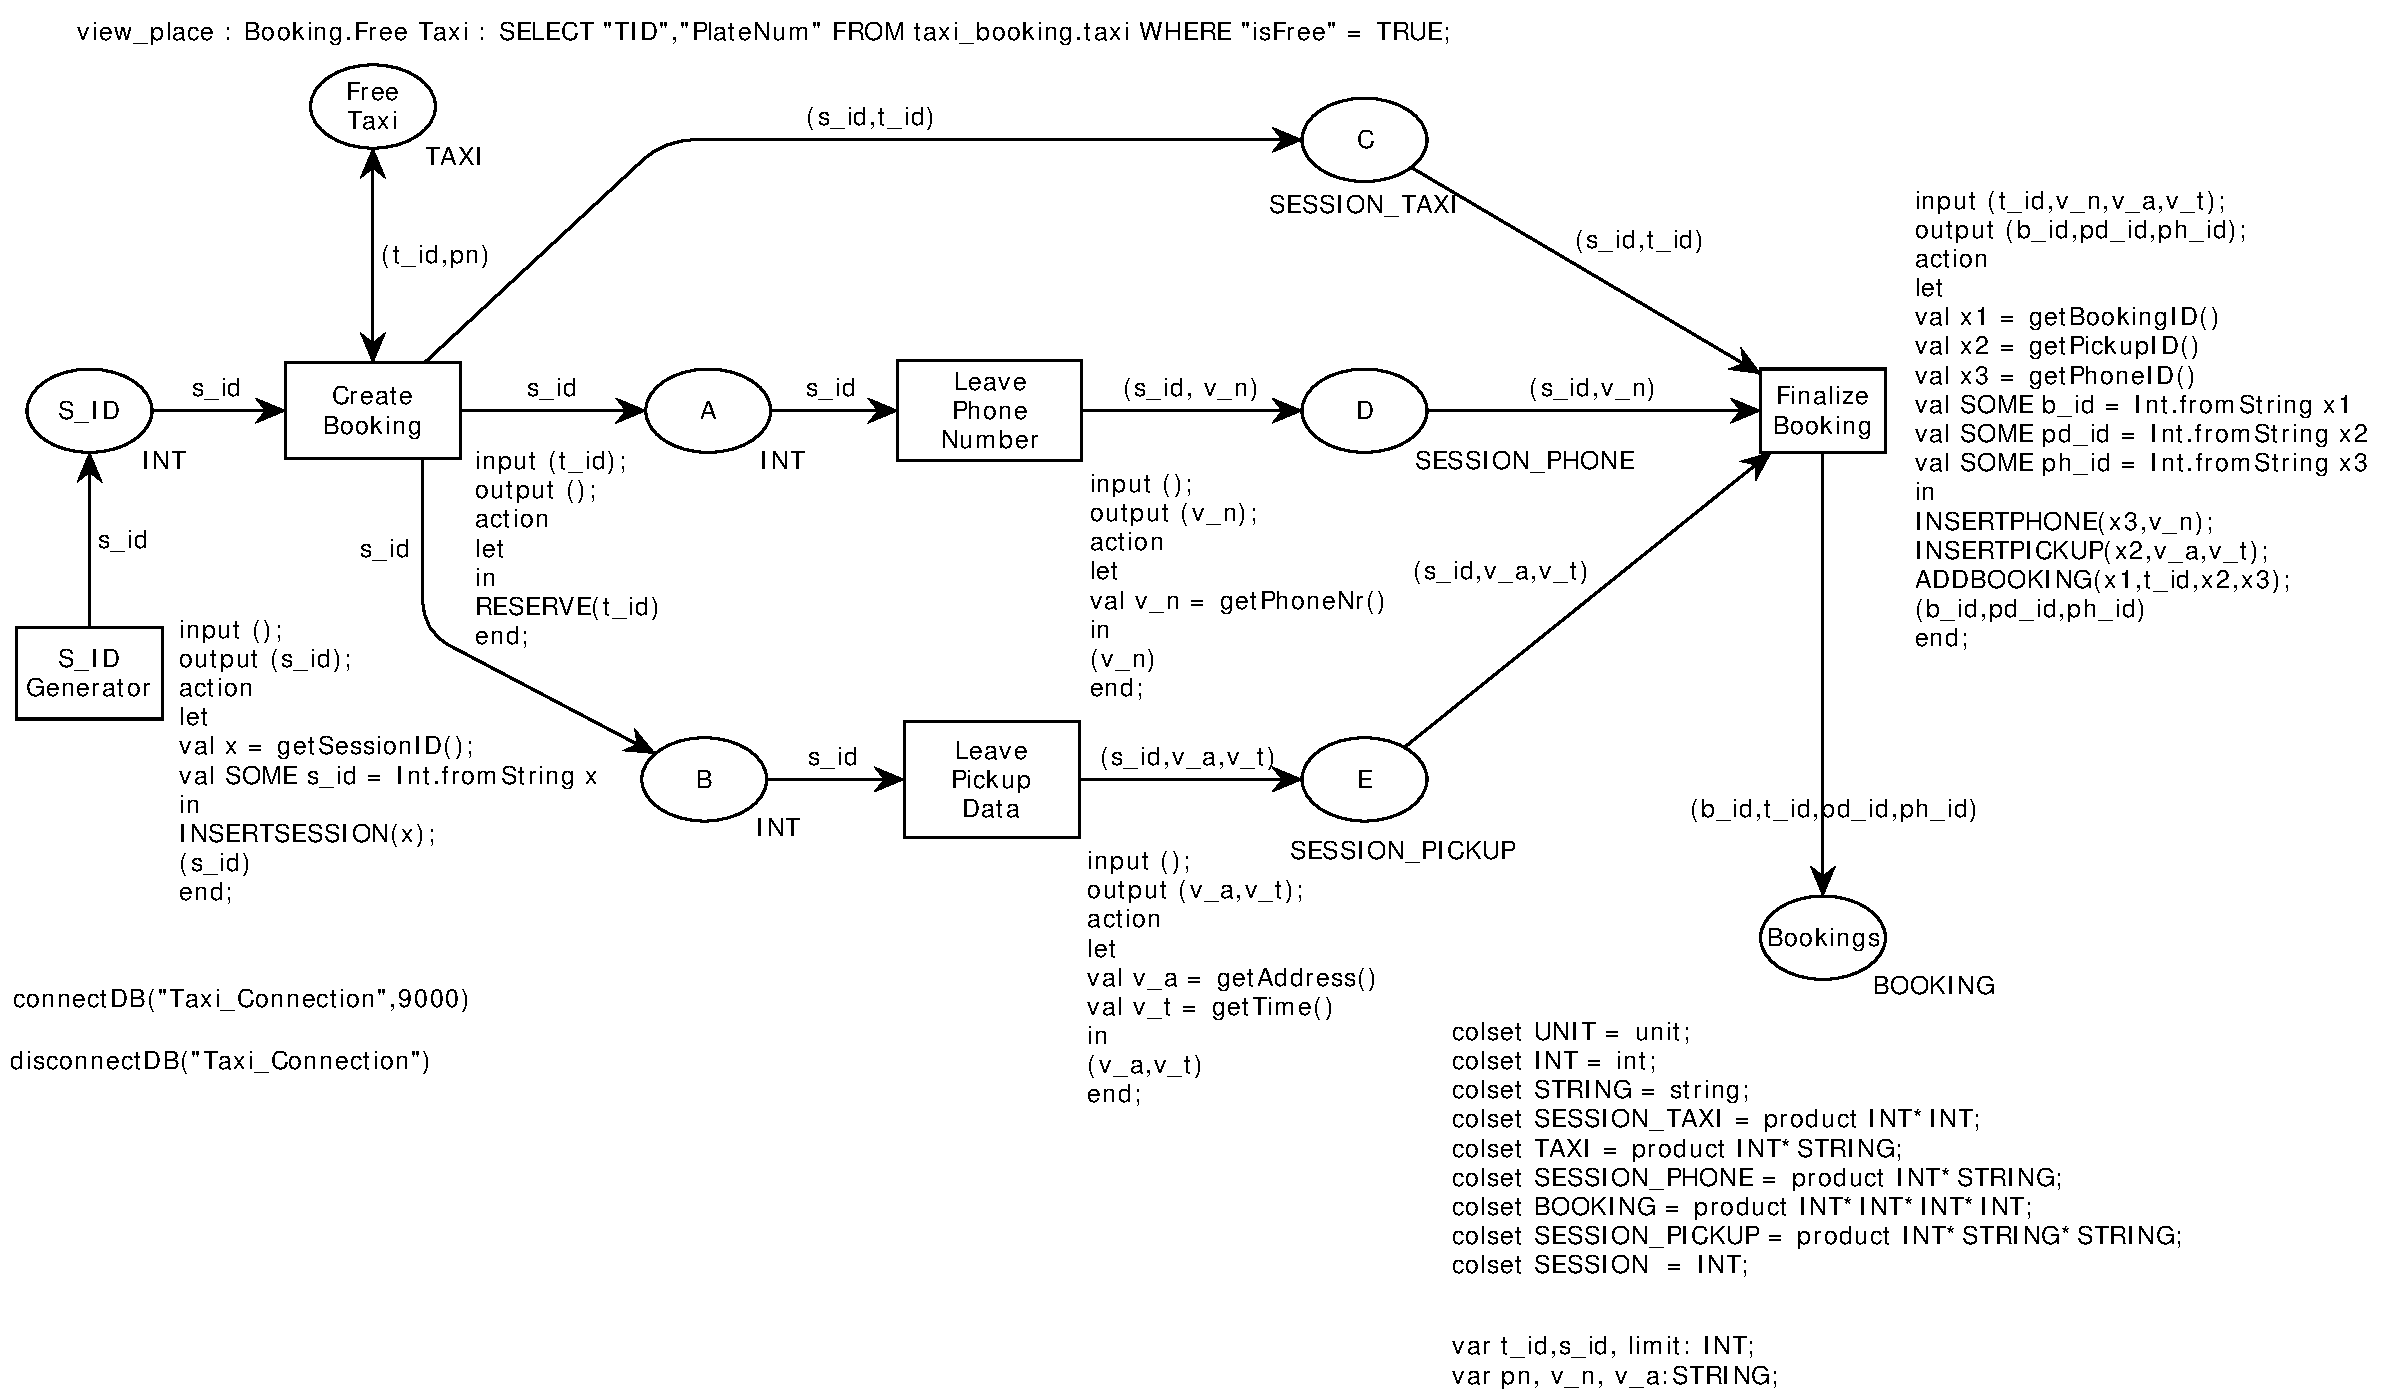
\includegraphics[scale = 0.35]{DBN_Impl_executable_model.pdf}
	\caption{Executable DB-net model for taxi booking}
	\label{fig:DBN_Impl_executable_model}
\end{figure}

\begin{figure}[!htbp]
	\centering
	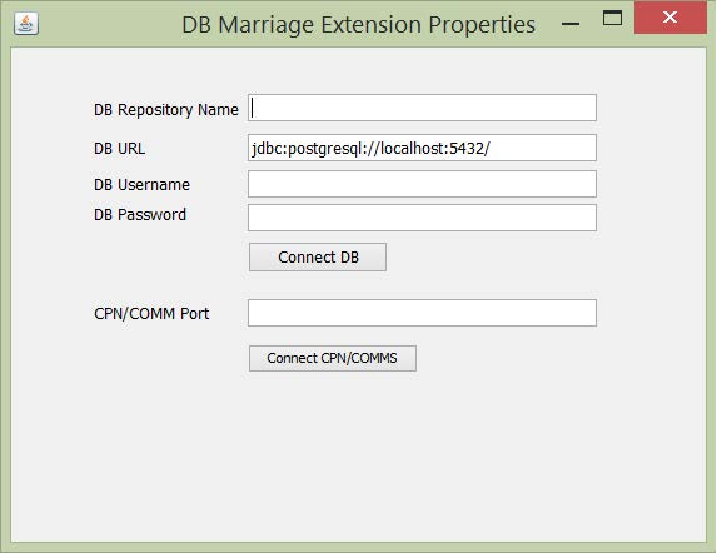
\includegraphics[scale = 0.75]{DBN_Impl_Extension_Dialog.pdf}
	\caption{Interface to provide connection parameters}
	\label{fig:DBN_Impl_Extension_Dialog}
\end{figure}

\subparagraph*{\textnormal{In order to execute actions in the transitions, we need to set up another connection using Comms/CPN. As a rule, in the attempt to establish a connection, the first handshake needs to be made using the Comms/CPN APIs and then the JAVA process can connect to the specified port. So, first we execute the \textit{connectDB} code, written in the text box, using the ML tool, then we provide the port number to the interface (see Figure \ref{fig:DBN_Impl_Extension_Dialog}) and finally we connect. Once the connection is successful, the user can play the token game using simulation tool box provided in the CPN Tools. In the net, whenever, a transition is fired, the view place automatically gets updated.}}

\subparagraph*{\textnormal{In this chapter, we discussed the implementation of DB-nets using CPN Tools extension and JAVA process. Using the mentioned modelling techniques, one can perform the simulation of DB-nets model in CPN Tools. In the next chapter, we will cover the analysis of DB-nets.}}

%%\begin{comment}
%\subsection{Architecture}
%\label{subsec:DBN_Impl_Architecture}
%\paragraph*{\textnormal{In this section, we present an idea for the implementation of different layers of DB-nets. In Figure \ref{fig:DBN_Impl_Mapping_Framework}, the DB-netlayers are mapped to their corresponding implementation paradigm. The persistence layer is modelled in PostgresSQL which is a relational database management system (RDBMS). The data logic layer is implemented as a JAVA application and for the control layer, we use CPN Tools.}}
%
%\begin{figure}[!htbp]
%	\centering
%	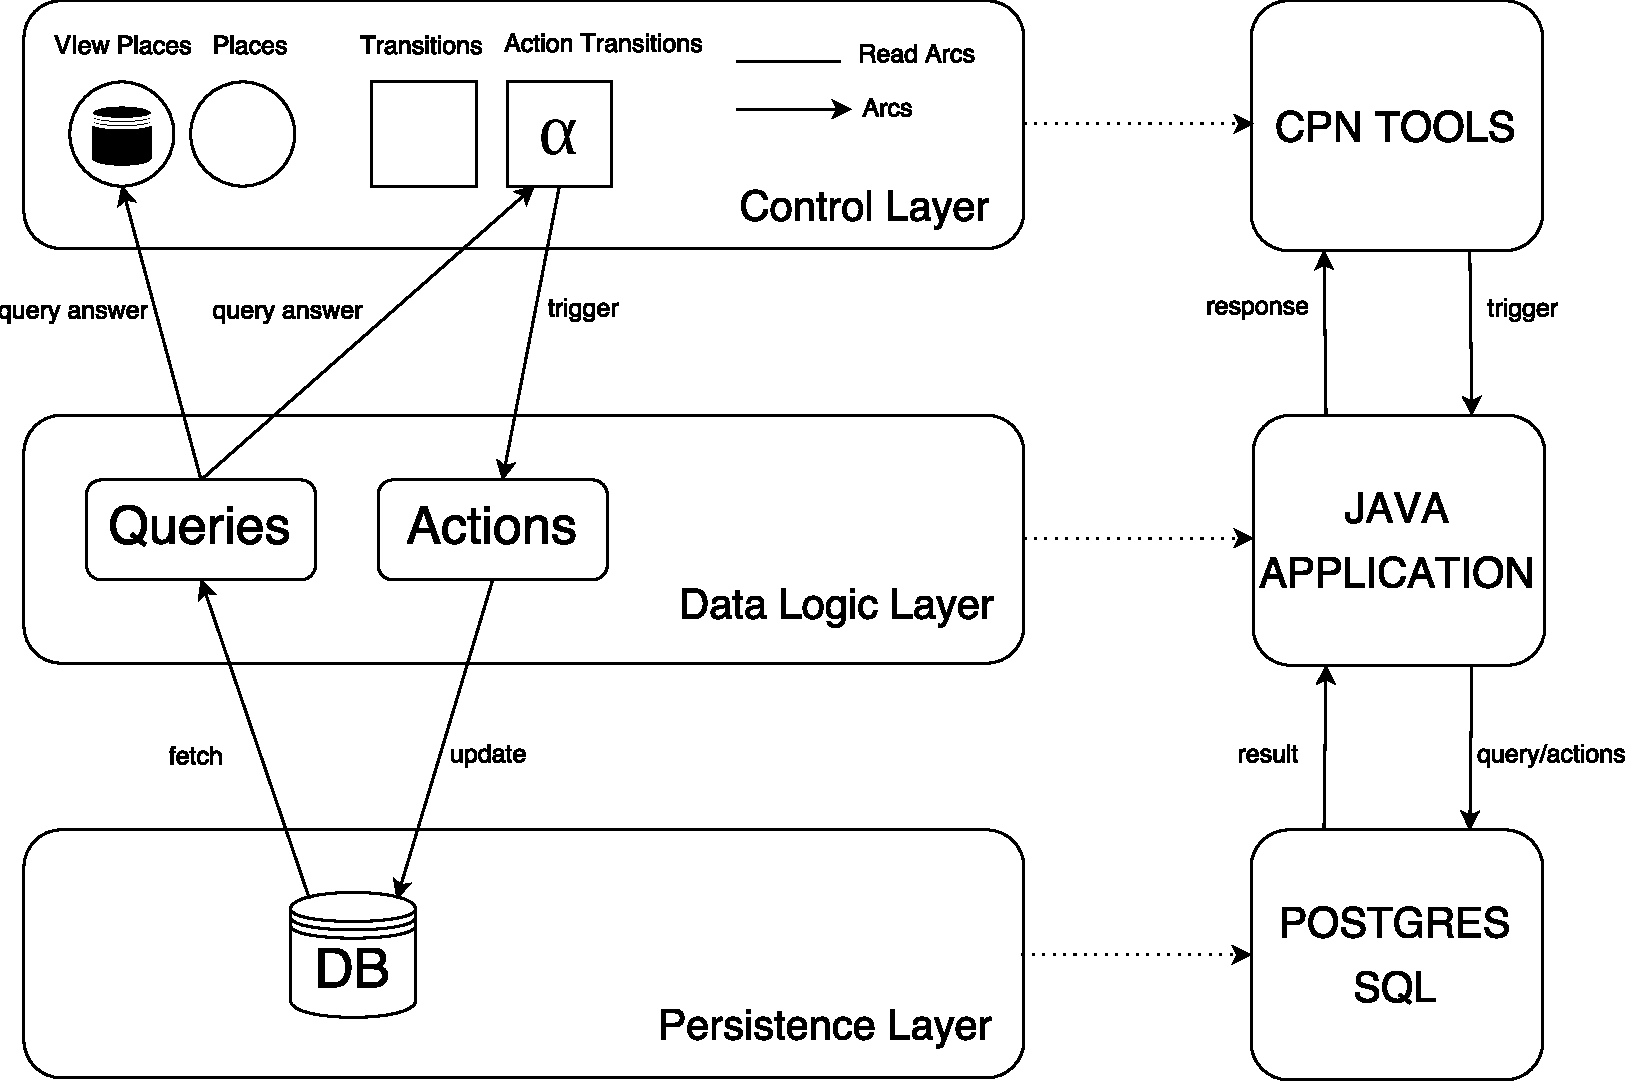
\includegraphics[scale = 0.35]{DBN_Impl_Mapping_Framework.pdf}
%	\caption{The mapping of db-net framework}
%	\label{fig:DBN_Impl_Mapping_Framework}
%\end{figure}
%
%\subparagraph*{\textnormal{The JAVA application comprises of the CPN Tools extension along with JAVA/CPN. JAVA/CPN allows JAVA processes to communicate with CPN Tools through Comms/CPN \footnote{Comms/CPN is a Standard ML library that augments Design/CPN with the necessary infrastructure to establish communication between CPN models and external processes. For source code of Comms/CPN, refer \cite{CPN_Tools_Comms/CPN}.} (refer \cite{gallasch2001comms}). The communication architecture between CPN Tools and JAVA/CPN is shown in Figure \ref{fig:DBN_Impl_CPNTools_Comms_JAVACPN_Comm}. CPN Tools use CPN-ML (a modified version of SML) as their programming language and Comms/CPN library is written in SML(compatible with CPN-ML). Comms/CPN use TCP/IP protocol to send/receive messages over a specified port. JAVA/CPN is a library, written in JAVA, is used to listen to send/receive messages through the specified port.}}
%
%\begin{figure}[!htbp]
%	\centering
%	
\includegraphics[scale = 0.35]{DBN_Impl_CPNTools_Comms_JAVACPN_Comm.pdf}
%	\caption{Communication between CPN Tools, Comms/CPN and JAVA/CPN}
%	\label{fig:DBN_Impl_CPNTools_Comms_JAVACPN_Comm}
%\end{figure}
%
%\subparagraph*{\textnormal{Figure \ref{fig:DBN_Impl_Java_App_Division} shows the framework through which the communication among different components takes place. Comms/CPN is used to connect to external environment/processes, which could possibly be web services etc, for data acquisition.\todo{AR:why for simplicity? AS:removed} Instead connecting to web services, we connect JAVA/CPN to database.\todo{AR: What did you want to say by that sentence? In our case Comms/CPN is just used to connect to DBs.\\AS:modified} We also modify JAVA/CPN and write our JAVA functions in order to facilitate data acquisition.\todo{how do you modify Comms/CPN? do you really expose your APIs like a web-service? it's just that I've never seen "expose" used in any other context but web services.\\AS:removed the exposed word} For example, while booking a taxi, when we fire \textit{Finalize Booking} transition, we add the booking with an id which is unique to the \textit{BOOKING} table, thus consulting the table for the ids which are not taken. Whereas, in order to receive the phone number of the customer, we don't need to consult the database and we use our function \textit{randomInt}.\todo{AR: randomInt is a function, right? also, try to come up with some special style for functions etc.\\AS: special style for functions?} In order to execute actions, one has to use the functions provided alongside JAVA/CPN. The query attached to a view place is processed by CPN Tools extension and the marking is returned as an answer to the corresponding query. For our use, we adopt the framework presented in Figure \ref{fig:DBN_Impl_Layer_Framework}.}}
%\begin{figure}[!htbp]
%	\centering
%	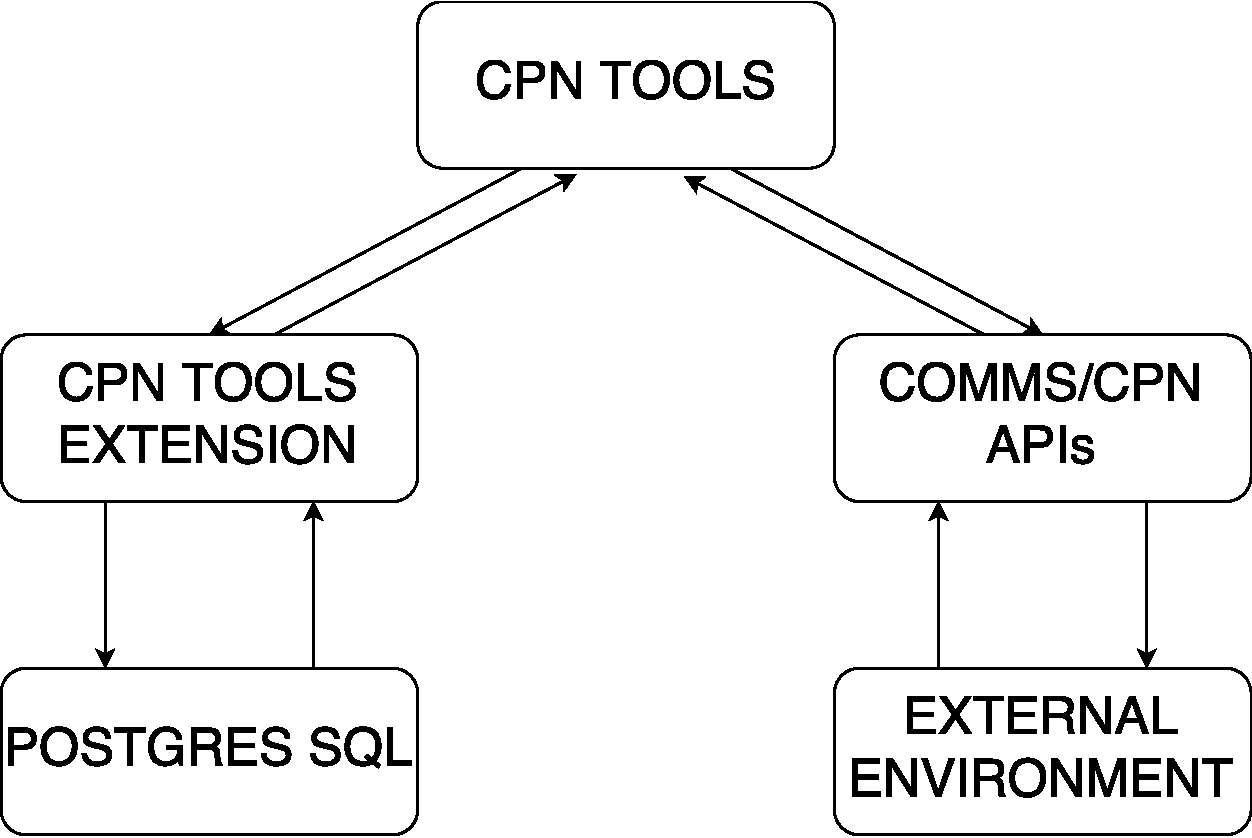
\includegraphics[scale = 0.35]{DBN_Impl_Java_App_Division.pdf}
%	\caption{Interconnectivity between different different components}
%	\label{fig:DBN_Impl_Java_App_Division}
%\end{figure}
%\begin{figure}[!htbp]
%	\centering
%	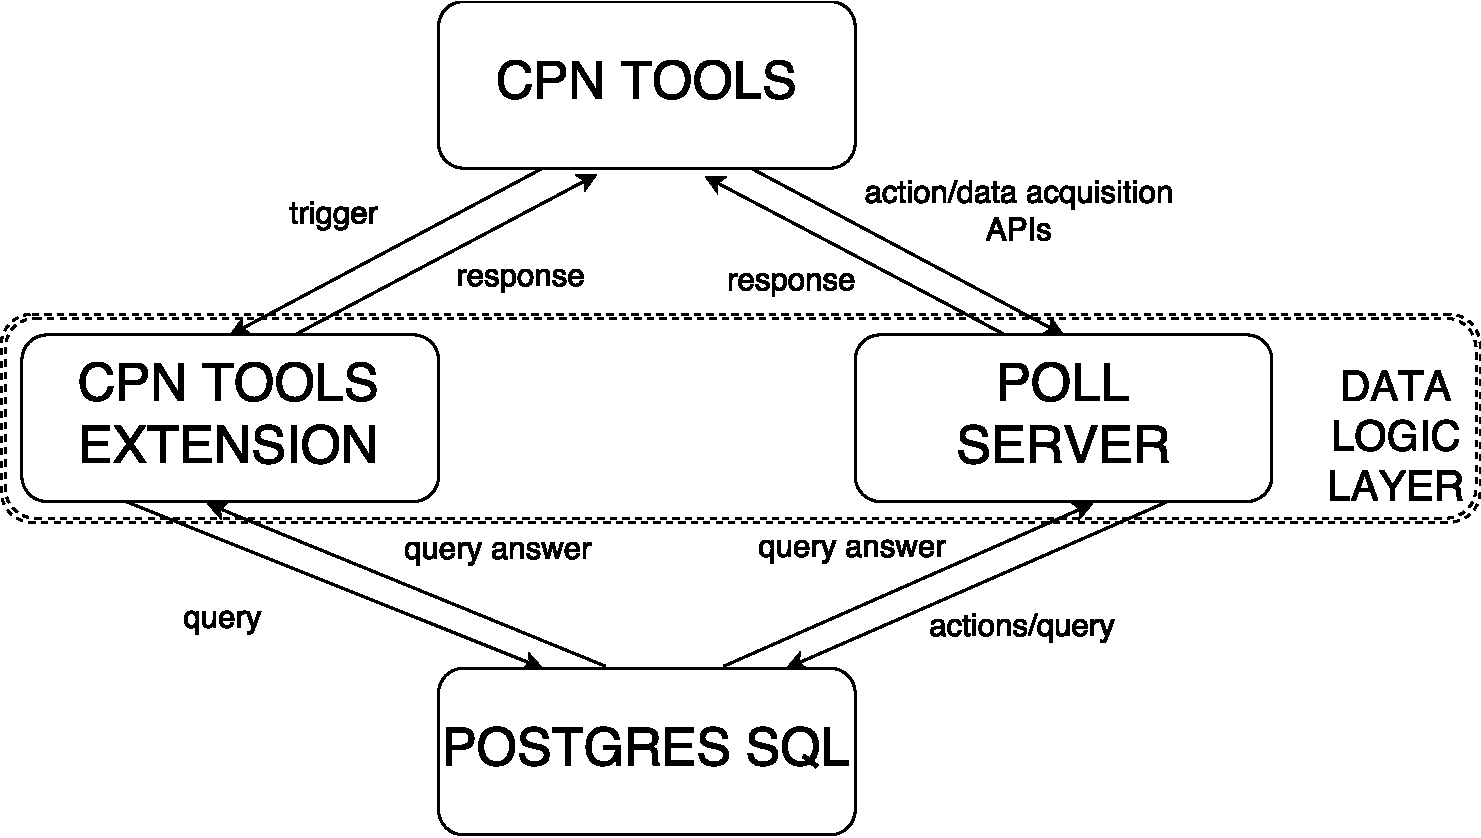
\includegraphics[scale = 0.35]{DBN_Impl_Layer_Framework.pdf}
%	\caption{Data logic layer division}
%	\label{fig:DBN_Impl_Layer_Framework}
%\end{figure}
%
%\section{Implementation}
%\label{sec:DBN_Impl_Impl}
%\subsection*{Persistence Layer}
%\label{subsec:DBN_Impl_persistence_layer}
%\paragraph*{\textnormal{The persistence layer is modelled in Postgres (an open source object-relational database management system, refer \cite{Postgres}). We name our database schema as \bdsq{taxi\_booking} (see Figure \ref{fig:DBN_Impl_Persistence_Layer}) which contains tables and constraints. The table \textit{session} contains the generated session ids for each booking session. The table \textit{taxi},\textit{phone} and \textit{pickup\_data} contains the information regarding taxi, customer's phone details and pickup details. Table \textit{booking} contains data related to the final booking. As indicated(see Figure \ref{fig:DBN_Impl_Persistence_Layer}), the relational schema also contains primary key and foreign key constraints. \todo{AR: fix the sentence\\AS: fixed}\todo{AR: first of all, you don't need to explain what SQL means. then, it's not enough to say that updates are performed using SQL. it's quit an obvious statement given that you are working with a relational DB. a certain update occurs after a corresponding action has been successfully executed. and then you discuss it in details later on.\\AS:fixed}}}
%
%\begin{figure}[!htbp]
%	\centering
%	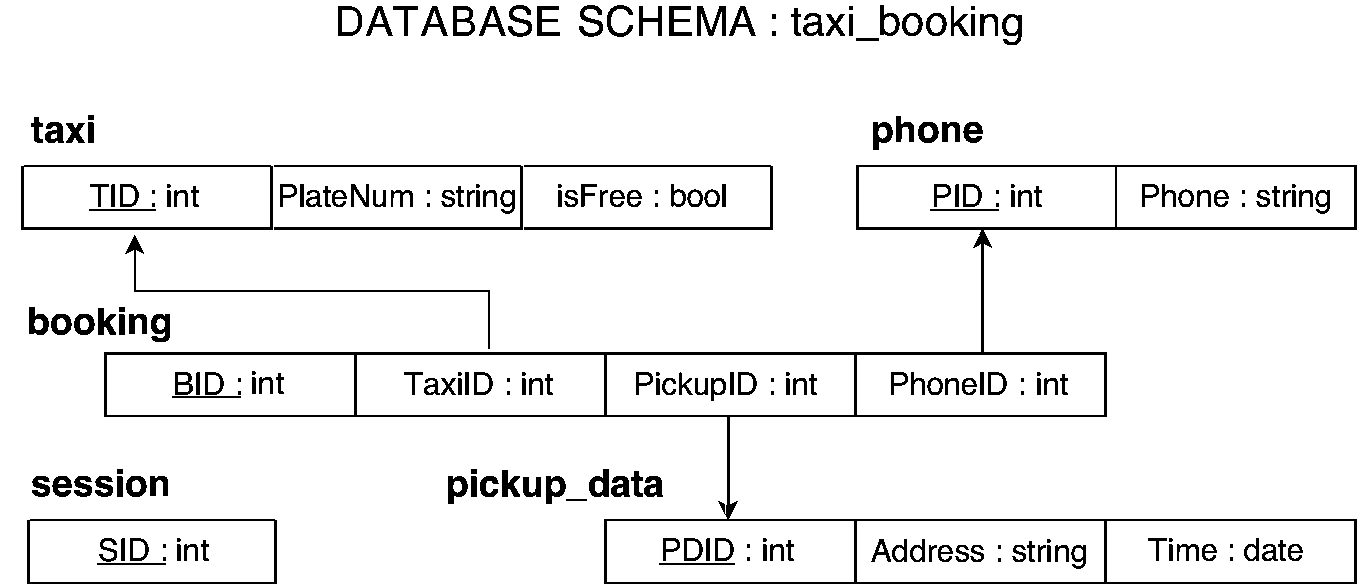
\includegraphics[scale = 0.45]{DBN_Impl_Persistence_Layer.pdf}
%	\caption{Database Schema for taxi booking example}
%	\label{fig:DBN_Impl_Persistence_Layer}
%\end{figure}
%
%\subsection*{Data Logic Layer and Control Layer}
%\label{subsec:DBN_Impl_control_layer}
%\paragraph*{\textnormal{Data logic layer is implemented as JAVA application and the control layer is implemented in CPN Tools. As shown in Figure \ref{fig:DBN_Impl_Java_App_Division} the data logic layer consists of two parts :
%		\begin{itemize}
%			\item CPN Tools extension
%			\item Comms/CPN APIs
%		\end{itemize}
%}}
%\subsubsection*{CPN Tools extension}
%\subparagraph*{\textnormal{In CPN Tools, the three major components are:
%		\begin{itemize}
%			\item GUI
%			\item Simulator
%			\item Extension
%\end{itemize}}}
%\subparagraph*{\textnormal{The modelling and execution of any CP nets depends on the interaction between GUI and Simulator. On the other hand, extensions are used to provide user-specific functionality in terms of simulation(execution) or modelling(GUI). \todo{all these pattern numbers are confusing. either one should present all the patterns in the appendix, or not even mention concrete references. AS: stuck to one} We design our extension on the communication pattern\footnote{Other communication patterns are mentioned in \cite{CPN_Tools_Extension}} presented in Figure \ref{fig:DBN_Impl_Extension_Communication_Pattern}.}}
%\begin{figure}[!htbp]
%	\centering
%	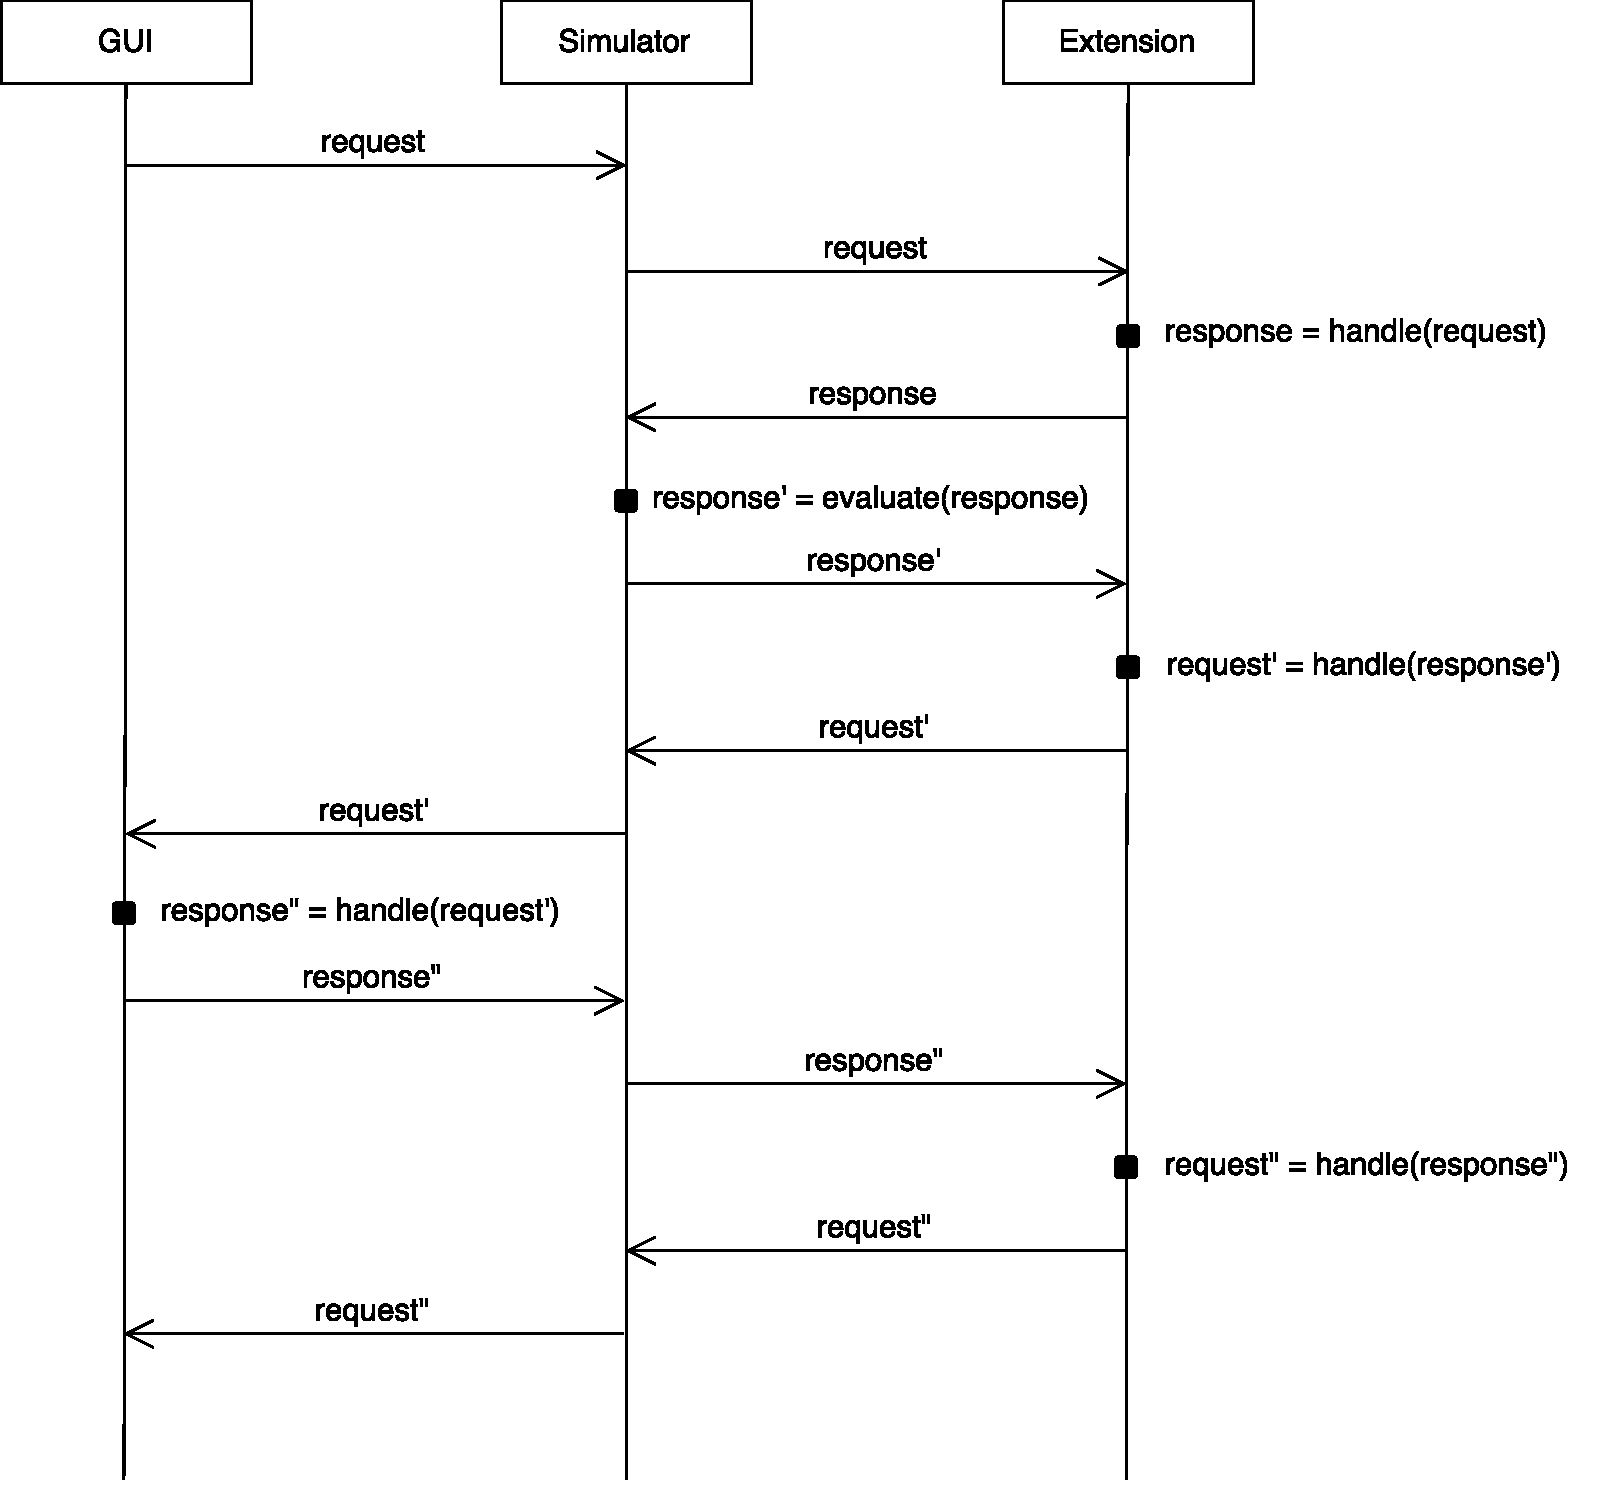
\includegraphics[scale = 0.40]{DBN_Impl_Extension_Communication_Pattern.pdf}
%	\caption{Communication Pattern of CPN Tools extensions}
%	\label{fig:DBN_Impl_Extension_Communication_Pattern}
%\end{figure}
%
%\subparagraph*{\textnormal{The responsibility of the extension is to look for changes in the DB-net model. \todo{fix this sentence}For example, changes related to modelling such as defining view places, declaring variables and colour sets, to execution events such as firing of transitions, the enabledness of transition etc., the extension listens to such events. Such \textit{requests}\footnote{We call events which is of our interests as \textit{requests}.}(modelling and execution)\todo{you should probably better define requests mentioned in Fig. 4.6} are passed from GUI to the extension via simulator. The extension takes appropriate response and passes on to the simulator. Simulator checks whether the response could be safely incorporated by the GUI i.e. the request should not bring CPN Tools to an inconsistent state,\todo{what does it mean "compatible with the GUI"?} and returns its evaluation to the extension. Once the evaluation is received, the extension handles the evaluated response and makes a request to the GUI to update. Once the request is incorporated/rejected by GUI, the response is sent to the extension. Extension handles the received response and gives the control back to the GUI. We will look at an example for this communication pattern later in the chapter.}} 
%
%\subparagraph*{\textnormal{The extension is also responsible for maintaining the connection with the database and performing queries over them. The whole working of the extension depends on the listening to the packets forwarded by the simulator. To know more about low level implementation of this extension, refer {\color{red} give reference to the documentation}.}}
%
%\subsubsection*{Modelling View Places}
%\subparagraph*{\textnormal{View places are drawn like normal places in CPN Tools. Also, view places carry SQL query along themselves. The syntax to define a view place is:}}
%\subparagraph*{}
%\begin{lstlisting}[showstringspaces=false, language = ML, caption = Syntax : view place, captionpos=b]
%view_place : <PageName.PlaceName> : <Query>
%\end{lstlisting}
%
%\subparagraph*{\textnormal{The above declaration should be written with \bdsq{Text} tool. For example, in Figure \ref{fig:DBN_Impl_Control_Layer}, the declaration for the view place is written as:
%}}
%\subparagraph*{}
%\begin{lstlisting}[showstringspaces=false, language = ML, caption = Syntax : view place, captionpos=b]
%view_place : Booking.Free_Taxi : SELECT "TID","PlateNum" FROM taxi_booking.taxi WHERE "isFree" = TRUE;
%\end{lstlisting}
%
%\begin{comment}
%For view places, the attached queries is written with the help of \bdsq{Text} Tool \todo{In appendix,Also define the regex for defining the view places} (provided by CPN Tools)\todo{I think that mentioning one of the tools here is a bit redundant}. The queries attached to action transitions or view places are written in SQL. One such part showing view places and action transitions in the taxi boking model is presented in Figure \ref{fig:DBN_Impl_Control_Layer}.\todo[inline]{Figure 4.5 demonstrates...} With the help of Text Tool (provided in the auxiliary palette)\todo{why so many details about tools from CPNTools? I think that if someone wants to use CPNTools, she will definitely find Text Tool.}, we make a statement declaring the view place along with the name of the place\todo{here you should explain better (without any footnotes) how one can define a view place} \footnote{The name of the view place is declared by adding the page name as the prefix (see Figure \ref{fig:DBN_Impl_Control_Layer}).}. In the figure\todo{which figure?}, the view place \textit{Free\_Taxi} is connected to the action transition \textit{Create Booking}. The query attached to the view place is:
%\end{comment}
%
%\begin{figure}[!htbp]
%	\centering
%	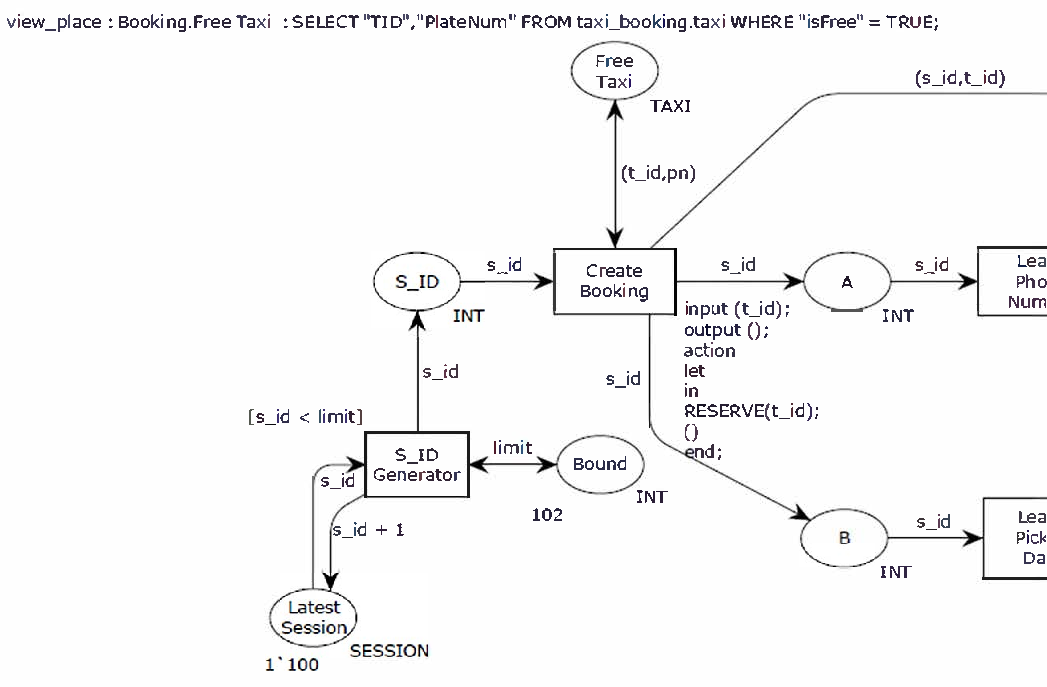
\includegraphics[scale = 0.60]{DBN_Impl_Control_Layer.pdf}
%	\caption{View Place, Action Transition and Read Arcs representation}
%	\label{fig:DBN_Impl_Control_Layer}
%\end{figure}
%
%\subparagraph*{\textnormal{Let's see the example of populating the view places using the communication pattern presented in Figure \ref{fig:DBN_Impl_Extension_Communication_Pattern}. When we declare a view place (see Figure \ref{fig:DBN_Impl_Control_Layer})\todo{are view places declared dynamically?}, the extension listens to the GUI and determines the declaration. In this case, the \textit{request} is passed from the GUI to the extension via simulator. The extension \textit{handles} the request and takes appropriate \textit{response} by fetching the marking(for the view place) from the database. However, at this stage, extension doesn't know if the markings are compatible with the colour set of the view place. In order to verify, if the marking is compatible to the colour set of the view place, the \textit{response} is passed to the simulator. The simulator evaluates (verification of the marking) the \textit{response} and provides its decision (\textit{response\textquotesingle}) to the extension whether the marking is compatible to the colour set of the view place. On receiving the evaluation, extension handles it and in case the marking is compatible, it creates a new request(\textit{request\textquotesingle}) to change the marking of the view place and passes on to the GUI via simulator. On receiving the new request, the GUI changes the marking of the view place. After incorporating the request (by changing the marking of view place), the GUI sends a response(\textit{response\textquotedbl}) to the extension whether the request (\textit{request\textquotesingle}) was successful or unsuccessful. Upon receiving the response, the extension handles it and gives back the control to the GUI.}}
%
%\subsubsection*{Modelling Action Transitions}
%\subparagraph*{\textnormal{The actions which are attached to the action transitions are modelled using ML functions. The code segment of transitions helps us in defining actions. The code segment has \textit{input}, \textit{output} and \textit{action} part. The input variables(the variables of interest) should be mentioned in the \textit{input} part and the fresh variables should mentioned in the \textit{output} part. The \textit{action} part has \textit{let\ldots in \ldots end} construct\footnote{This construct is similar to the construct for ML functions.}. The data for the fresh variables is acquired in the \textit{let} part whereas \textit{in} part contains \textit{actions}. Just before the \textit{end} part, the fresh variables(if any) should be written within parentheses in order corresponding to the variables in the \textit{output} part. In Figure \ref{fig:DBN_Impl_Control_Layer}, the \textit{let\ldots in \ldots end} part of the \textit{Create Booking} transition is written as:}}
%
%\subparagraph*{}
%
%\begin{lstlisting}[showstringspaces=false, language = ML, caption = Code Segment : \textit{Create Booking} transition, captionpos=b, label = lst:DBN_Impl_Create_Booking_code_segment, numbers=left,
%stepnumber=1]
%input (t_id);
%output ();
%action
%let
%in
%RESERVE(t_id);
%()
%end;
%\end{lstlisting}
%
%\subparagraph*{\textnormal{The \textit{Create Booking} transition has \textit{RESERVE} action, which takes the selected taxi id as parameter and reserves it. The \textit{RESERVE} action is defined as an ML function:
%}}
%
%\subparagraph*{}
%
%\begin{lstlisting}[showstringspaces=false, language = ML, caption = RESERVE action, captionpos=b, label = lst:DBN_Impl_RESERVE_action_query]
%fun RESERVE(t_id) = exQuery("UPDATE taxi_booking.taxi SET \"isFree\" = FALSE WHERE \"TID\" ="^ Int.toString t_id^";");
%\end{lstlisting}
%
%\subparagraph*{\textnormal{\textit{exQuery} is an ML function which takes the query\footnote{In the query, (see Listing \ref{lst:DBN_Impl_RESERVE_action_query}), the {\textbackslash \textquotedbl} symbol is used in ML to represent double quotes in string where as $\string^$ symbol is used to concatenate two strings.} as a parameter and passes it to Comms/CPN for execution.\todo{AR:passes what? \\ AS:reframed} For example, for $t\_id = 47552$, the query to be passed would be :}}
%
%\subparagraph*{}
%\begin{lstlisting}[showstringspaces=false, language = SQL, caption = RESERVE action query simplification, captionpos=b, label = lst:DBN_Impl_RESERVE_action_query_ex]
%UPDATE taxi_booking.taxi SET "isFree" = FALSE WHERE "TID" = 47552;
%\end{lstlisting}
%
%\subparagraph*{\textnormal{The \textit{exQuery} function internally calls the Comms/CPN APIs, thus passing actions through Comms/CPN to the database. In order to execute actions attached to action transitions and acquiring data from the external environment we use Comms/CPN. Comms/CPN provide a set of APIs which are:
%		\begin{enumerate}
%			\item \textit{openConnection} - allows users to connect to external process as a client. It takes three parameters, the first is the connection name which is a unique identifier, the second is the host name and the third is the port number.  
%			\item \textit{acceptConnection} - allows external processes to connect to CPN Tools GUI. It takes two parameters, first is the connection name which is a unique identifier and the second one is the port number where the connection needs to be established.
%			\item \textit{send} - allows users to send any type of data to external processes. It takes three parameters, the first is the connection identifier followed by the data to be sent. The last parameter is the encoding function which is used to encode the data to a byte stream.
%			\item \textit{receive} - allows users to receive any type of data from external processes.It takes two parameters, the first is the connection identifier followed by a parameter specifying the decoding function to  decode the received data(in byte stream) from the connection.
%			\item \textit{closeConnection} - allows users to close a connection. Takes a single parameter which specifies name of the connection to be closed.
%\end{enumerate}}}
%
%\subparagraph*{\textnormal{In our case, we don't use \textit{openConnection} since we don't work in a remote architecture. \todo{AR: you should explain what does it mean to be a client here.\\AS:Here I am really not sure, it is in the sense that CPNTools is running on one machine and the COMMS server is running on other machine, and if we want to connect them remotely. I never tried this architecture, involves some kind of networking.}The \textit{send} and \textit{receive} APIs send and receive data in \textit{string} data-type. \textit{closeConnection} closes the connection. In order to set up the connectivity with Comm/CPN and CPN Tools, we create ML function which calls Comms/CPN APIs. For example, we create connectDB\footnote{While calling \textit{acceptConnection} we assume that the connection name is \bdsq{Taxi\_Connection}. We will use this connection name through out our example.} and disconnectDB function in ML which can be defined as:}}
%\subparagraph*{}
%\begin{lstlisting}[showstringspaces=false, language = ML, caption = Accept/Close connection functions, captionpos=b, label = lst:DBN_Impl_acc_close_conn_func]
%fun connectDB(connName, port) = acceptConnection(connName, port);
%fun disconnectDB(connName) = closeConnection(connName);
%\end{lstlisting}
%
%\subparagraph*{\textnormal{We encapsulate the name of the functions for data acquisition (\textit{funcAPI}) in a string and send it using the Comms/CPN APIs\footnote{We modify Comms/CPN source code and add our functions}. On receiving the string, the decoder decodes the string and calls the corresponding data acquisition APIs. The set of ML functions\todo{you need to explain that comms works through ML. moreover, the function you define below are of two different kinds. getFromDB and exQuery are "canonical" functions that remain intact for every db-net model, while getRandom is specific for your concrete example.}\footnote{In order to make our functions consistent with the provided Comms/CPN APIs we use string as the data type while passing the parameters.} which internally calls the Comms/CPN APIs are:
%		\begin{enumerate}
%			\item \textit{getRandom} - takes two parameters: \textit{funcAPI} and \textit{length}. The \textit{funcAPI} can be either \textit{randomInt}, \textit{randomString} or \textit{randomTime}. Based on the \textit{funcAPI}, data logic layer decides which function should be called and returns the result.
%			\item \textit{getFromDB} - takes four parameters: \textit{tableName}, \textit{columnName}, \textit{funcAPI} and \textit{length}. Currently the supported funcAPI is \bdsq{getFromDB} to get a unique identifier of given length for the specified \textit{tableName} and \textit{columnName}.
%			\item \textit{exQuery} - takes two parameters: \textit{funcAPI} and \textit{query}. Currently the supported funcAPI is \bdsq{exQuery} to execute the given query.
%\end{enumerate}}}
%
%\subparagraph*{\textnormal{The use of \textit{getRandom} and \textit{getFromDB} is optional and it depends on the requirement of the modeller but in order to execute queries, one should use \textit{exQuery}. The ML function for \textit{exQuery}, which can be used in the \textit{RESERVE} action mentioned in the Listing \ref{lst:DBN_Impl_RESERVE_action_query}, is:}}
%
%\subparagraph*{}
%\begin{lstlisting}[showstringspaces=false, language = ML, caption = exQuery function, captionpos=b, label = lst:DBN_Impl_exquery_func]
%fun exQuery(funcAPI, query) = ConnManagementLayer.send("Taxi_Connection", funcAPI^"?"^query, stringEncode);
%\end{lstlisting}
%
%\subparagraph*{\textnormal{The \bdsq{?}\todo{in general, a question mark is not the best solution due to ambiguities that my rise while using different SQL dialects. AS: which symbol should I use? Can you give me examples of ambiguities? I have heard about "?" being used in SPARQL} sign in the function is used to provide a marker to the data acquisition functions which helps in parsing the string received from the Comms/CPN.\footnote{The first parameter should be funcAPI, followed by other parameters separated by \bdsq{?}.} Using the example given in Listing \ref{lst:DBN_Impl_RESERVE_action_query_ex}, calling \textit{exQuery} can be seen as :}}
%
%\subparagraph*{}
%\begin{lstlisting}[showstringspaces=false, language = SQL, caption = exQuery Example, captionpos=b, label = lst:DBN_Impl_exquery_func_ex]
%ConnManagementLayer.send(Taxi_Connection, exQuery?UPDATE taxi_booking.taxi SET "isFree" = FALSE WHERE "TID" = 47552;, stringEncode);
%\end{lstlisting}
%
%\subparagraph*{\textnormal{Other functions such as \textit{getFromDB} and \textit{getRandom} can be written in ML as:}}
%
%\subparagraph*{}
%
%\begin{lstlisting}[showstringspaces=false, language = ML, caption = Data Acquisition Functions, captionpos=b, label = lst:DBN_Impl_data_acq_functions]
%fun getFromDB(funcAPI, t_name, c_name, length) =
%(ConnManagementLayer.send("Taxi_Connection", "getFromDB"^"?"^t_name^"?"^c_name^"?"^funcAPI^"?"^length, stringEncode);
%ConnManagementLayer.receive("Taxi_Connection", stringDecode));
%fun getRandom(funcAPI, length) = (ConnManagementLayer.send("Taxi_Connection", "getRandom"^"?"^funcAPI^"?"^length, stringEncode);
%ConnManagementLayer.receive("Taxi_Connection", stringDecode));
%\end{lstlisting}
%
%\begin{comment}
%content...
%
%\subsection{Data Logic Layer}
%\paragraph*{\textnormal{As shown in Figure \ref{fig:DBN_Impl_Java_App_Division} the data logic layer consists of two parts :
%\begin{itemize}
%\item CPN Tools extension
%\item Comms/CPN APIs
%\end{itemize}
%}}
%\subsubsection*{CPN Tools extension}
%\subparagraph*{\textnormal{In CPN Tools, the three major components are:
%\begin{itemize}
%\item GUI
%\item Simulator
%\item Extension
%\end{itemize}}}
%\subparagraph*{\textnormal{The modelling and execution of any CP nets depends on the interaction between GUI and Simulator. On other hand, extensions are used to provide user-specific functionality in terms of simulation(execution) or modelling(GUI). There are many communication patterns presented in \cite{CPN_Tools_Extension}, and we adopt a mixture of pattern 6,7 and 8 \todo{AR: all these pattern numbers are confusing. either one should present all the patterns in the appendix, or not even mention concrete references.\\AS:Removed} and design our extension on the pattern\footnote{Although, the pattern resembles to the pattern 9b, mentioned in \cite{CPN_Tools_Extension}, but it differs slightly from it.} presented in Figure \ref{fig:DBN_Impl_Extension_Communication_Pattern}.}}
%\begin{figure}[!htbp]
%\centering
%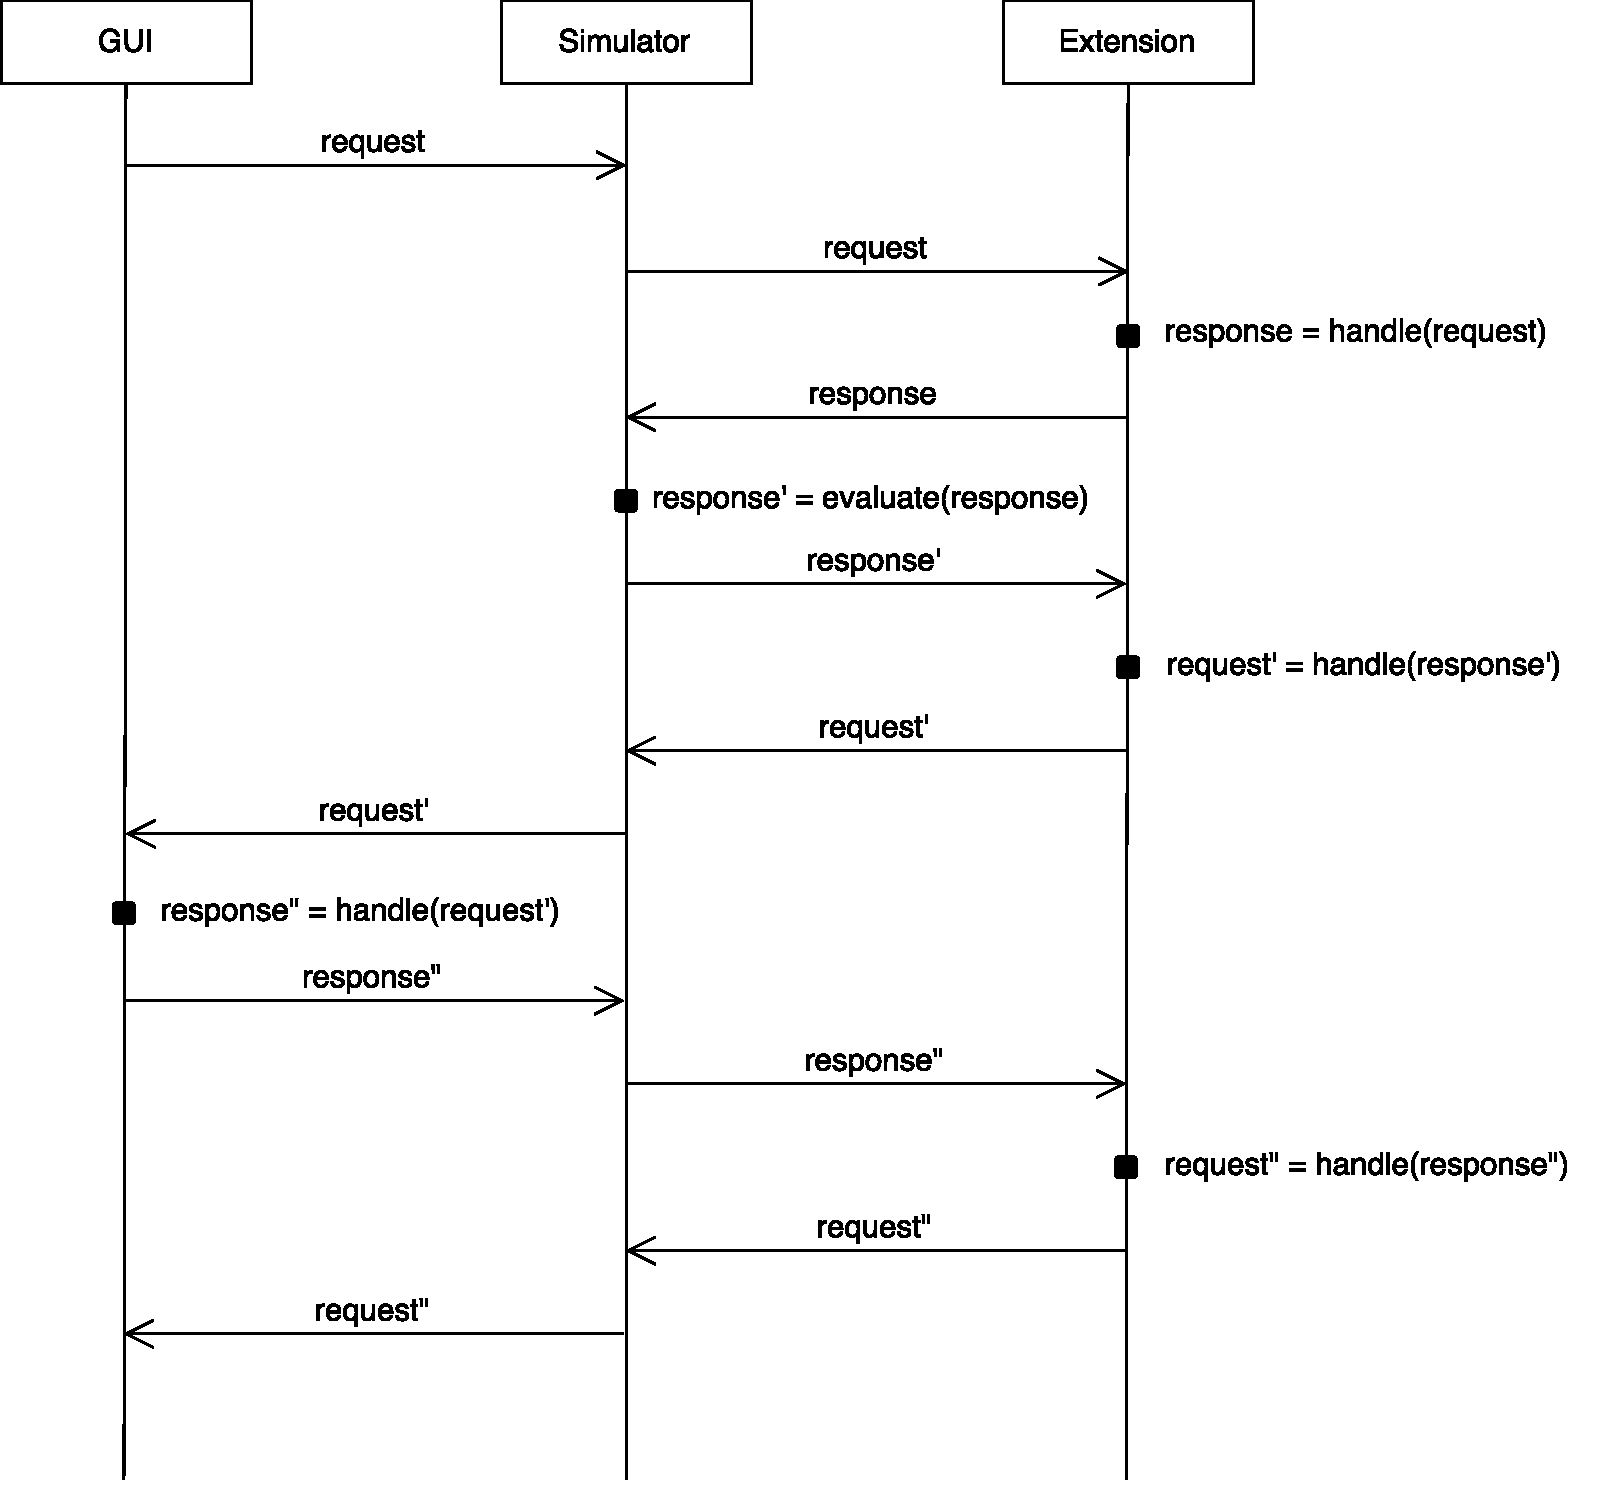
\includegraphics[scale = 0.40]{DBN_Impl_Extension_Communication_Pattern.pdf}
%\caption{Communication Pattern of CPN Tools extensions}
%\label{fig:DBN_Impl_Extension_Communication_Pattern_temp}
%\end{figure}
%
%\subparagraph*{\textnormal{The responsibility of the extension is to look for changes in the DB-net model. \todo{fix this sentence}For example, changes related to modelling such as defining view places, declaring variables and colour sets, to execution events such as firing of transitions, the enabledness of transition etc., the extension listens to such events. Such \textit{requests}\footnote{We call the events which is of our interests a \textit{requests}.}(modelling and execution)\todo{you should probably better define requests mentioned in Fig. 4.6} are passed from GUI to the extension via simulator. The extension takes appropriate response and passes on to the simulator. Simulator checks whether the response could be safely incorporated by the GUI i.e. the request should not bring CPN Tools to an inconsistent state,\todo{what does it mean "compatible with the GUI"?} and returns its evaluation to the extension. Once the evaluation is received, the extension handles the evaluated response and makes a request to the GUI to update. Once the request is incorporated/rejected by GUI, the response is sent to the extension. Extension handles the received response and gives the control back to the GUI.}}
%
%\subparagraph*{\textnormal{For instance, let's see the example of populating the view places using the communication pattern presented in Figure \ref{fig:DBN_Impl_Extension_Communication_Pattern}. When we declare a view place (see Figure \ref{fig:DBN_Impl_Control_Layer})\todo{are view places declared dynamically?}, the extension listens to the GUI and determines the declaration. In this case, the request is passed from the GUI to the extension via simulator. The simulator \textit{handles} the request and takes appropriate \textit{response} by fetching the marking(for the view place) from the database. This \textit{response} is passed to the simulator to check whether the marking is compatible to the view place (if the marking matches the colour set of the view place). The simulator evaluates the \textit{response} and provides its decision (\textit{response\textquotesingle}) to the extension. Extension creates a new request(\textit{request\textquotesingle}) to change the marking of the view place and passes on to the GUI. On receiving the new request, the GUI changes the marking of the view place. After incorporating the request (by changing the markings of view places), the GUI sends a response(\textit{response\textquotedbl}) to the extension whether the request (\textit{request\textquotesingle}) was successful or unsuccessful. Upon receiving the response, the extension handles it and gives back the control to the GUI.}}
%
%\subparagraph*{\textnormal{Apart from populating view places, extension is also responsible for maintaining the connection with the database and performing queries over them. The whole working of the extension depends on the listening to the packets forwarded by the simulator. To know more about low level implementation of this extension, refer {\color{red} give reference to the documentation}.}}
%
%\subsubsection{Comms/CPN APIs}
%\subparagraph*{\textnormal{In order to execute actions attached to action transitions and acquiring data from the external environment we use Comms/CPN. Comms/CPN provide a set of APIs which are:
%\begin{enumerate}
%\item \textit{openConnection} - allows users to connect to external process as a client. It takes three parameters, the first is the connection name which is a unique identifier, the second is the host name and the third is the port number.  
%\item \textit{acceptConnection} - allows external processes to connect to CPN Tools GUI. It takes two parameters, first is the connection name which is a unique identifier and the second one is the port number where the connection needs to be established.
%\item \textit{send} - allows users to send any type of data to external processes. It takes three parameters, the first is the connection identifier followed by the data to be sent. The last parameter is used to encode the data to a byte stream.
%\item \textit{receive} - allows users to receive any type of data from external processes.It takes two parameters, the first is the connection identifier followed by the parameter to  decode the received data(in byte stream) from the connection.
%\item \textit{closeConnection} - allows users to close a connection. Takes a single parameter which specifies name of the connection to be closed.
%\end{enumerate}}}
%\subparagraph*{\textnormal{In our case, we don't use \textit{openConnection} since we don't need to be a client. \todo{AR: you should explain what does it mean to be a client here.\\AS:Here I am really not sure, it is in the sense that CPNTools is running on one machine and the COMMS server is running on other machine, and if we want to connect them remotely. I never tried this architecture, involves some kind of networking.}. The send and receive APIs send and receive data in \textit{string} data-type. We encapsulate the name of required APIs for data acquisition (\textit{funcAPI}) in a string and send it using the Comms/CPN APIs\footnote{We modify Comms/CPN source code and add our APIs}. On receiving the string, the decoder decodes the string and calls the corresponding data acquisition APIs. The set of ML functions\todo{you need to explain that comms works through ML. moreover, the function you define below are of two different kinds. getFromDB and exQuery are "canonical" functions that remain intact for every db-net model, while getRandom is specific for your concrete example.}\footnote{In order to make our APIs consistent with the provided Comms/CPN APIs we use string while passing the parameters.} which internally calls the Comms/CPN APIs are:
%\begin{enumerate}
%\item \textit{getRandom} - takes two \textbf{string} parameters: \textit{funcAPI} and \textit{length}. The \textit{funcAPI} can be either \bdsq{randomInt} or \bdsq{randomString}. Based on the \textit{funcAPI}, data logic layer decides which function should be called and returns the result.
%\item \textit{getFromDB} - takes four parameters: \textit{tableName}, \textit{columnName}, \textit{funcAPI} and \textit{length}. Currently the supported funcAPI is \bdsq{getFromDB} to get a unique identifier of given length for the specified \textit{tableName} and \textit{columnName}.
%\item \textit{exQuery} - takes two parameters: \textit{funcAPI} and \textit{query}. Currently the supported funcAPI is \bdsq{exQuery} to execute the given query.
%\end{enumerate}}}
%
%\subparagraph*{\textnormal{
%\todo{you have to explain briefly before how to make comms work in a CPN model using ML} In order to create a connection with external applications using Comms/CPN, we create ML function with connection parameters. Similarly, we create an ML function for closing the connection. These two functions can be written as:}}
%
%\subparagraph*{}
%\begin{lstlisting}[showstringspaces=false, language = ML, caption = Accept/Close connection functions, captionpos=b, label = lst:DBN_Impl_acc_close_conn_func]
%fun connectDB(connName,port) = acceptConnection(connName,port);
%fun disconnectDB(connName) = closeConnection(connName);
%\end{lstlisting}
%
%\subparagraph*{\textnormal{While calling \textbf{acceptConnection} we assume that the connection name is \bdsq{Taxi\_Connection}\footnote{We will use this connection name through out our example.}.We create ML functions in CPN Tools, which encapsulates the required APIs(of the data logic layer) in a string and uses Comms/CPN APIs for sending or receiving. For example, the RESERVE action mentioned in the Listing \ref{lst:DBN_Impl_RESERVE_action_query}, the function \textit{exQuery} is written in ML (in CPN tools) as:
%}}
%
%\subparagraph*{}
%\begin{lstlisting}[showstringspaces=false, language = ML, caption = exQuery functions, captionpos=b, label = lst:DBN_Impl_exquery_func]
%fun exQuery(funcAPI,query) = ConnManagementLayer.send("Taxi_Connection",funcAPI^"?"^query,stringEncode);
%\end{lstlisting}
%
%\subparagraph*{\textnormal{The \bdsq{?}\todo{in general, a question mark is not the best solution due to ambiguities that my rise while using different SQL dialects} sign in the function is used to provide a marker to the data acquisition functions which helps in parsing the string received from the Comms/CPN.\footnote{The first parameter should be funcAPI, followed by other parameters separated by \bdsq{?}.} Using the example given in Listing \ref{lst:DBN_Impl_RESERVE_action_query_ex}, calling \textit{exQuery} can be seen as :}}
%
%\subparagraph*{}
%\begin{lstlisting}[showstringspaces=false, language = SQL, caption = exQuery Example, captionpos=b, label = lst:DBN_Impl_exquery_func_ex]
%ConnManagementLayer.send("Taxi_Connection","exQuery?UPDATE taxi_booking.taxi SET "isFree" = FALSE WHERE "TID" = 47552;",stringEncode);
%\end{lstlisting}
%
%\subparagraph*{\textnormal{In order to acquire data from the database, we use \textit{getFromDB} function, whereas to acquire random data for fresh variables, we use \textit{getRandom}. These functions can also be written in ML as:}}
%
%\subparagraph*{}
%
%\begin{lstlisting}[showstringspaces=false, language = ML, caption = Data Acquisition Functions, captionpos=b, label = lst:DBN_Impl_data_acq_functions]
%fun getFromDB(t_name, c_name,funcAPI,length) =
%(ConnManagementLayer.send("Taxi_Connection","getFromDB"^"?"^t_name^"?"^c_name^"?"^funcAPI^"?"^length,stringEncode);
%ConnManagementLayer.receive("Taxi_Connection",stringDecode));
%fun getRandom(funcAPI, length) = (ConnManagementLayer.send("Taxi_Connection","getRandom"^"?"^funcAPI^"?"^length,stringEncode);
%ConnManagementLayer.receive("Taxi_Connection",stringDecode));
%\end{lstlisting}
%
%\subparagraph*{\textnormal{We recommend modellers to use the given functions(Listing \ref{lst:DBN_Impl_acc_close_conn_func}, \ref{lst:DBN_Impl_exquery_func}, \ref{lst:DBN_Impl_data_acq_functions}) in order to use the APIs provided in the data logic layer\footnote{One can also create their own functions and APIs in the data logic layer and use them}.}}
%\end{comment}
%
%\section{DB-nets executable example}
%\label{sec:DBN_impl_example}
%
%\paragraph*{\textnormal{Figure \ref{fig:DBN_Impl_executable_model} represents an executable DB-net model of the taxi booking example modelled in CPN Tools. Note that the extension is always connected with the CPN Tools and is listening to the events. We assume that the connection between the database and the data logic layer is already established and the marking of the view place is fetched by the extension. Now, we try to establish connection between CPN Tools and the external environment using Comms/CPN APIs. Using the ML extension in CPN Tools(to execute a text as ML code), we execute the function \textit{connectDB} and \textit{disconnectDB}. We specify the connection name to be \bdsq{Taxi\_Connection}\footnote{By assuming this connection name through out the example, we refrain from passing the connection name to every function.} and the port to be \bdsq{9000}. The functions are written as:}}
%
%\subparagraph*{}
%\begin{lstlisting}[showstringspaces=false, language = ML, caption = Connection Setup, captionpos=b, label = lst:DBN_Impl_connection_setup]
%connectDB("Taxi_Connection",9000)
%disconnectDB("Taxi_Connection")
%\end{lstlisting}
%
%\begin{figure}[!htbp]
%	\centering
%	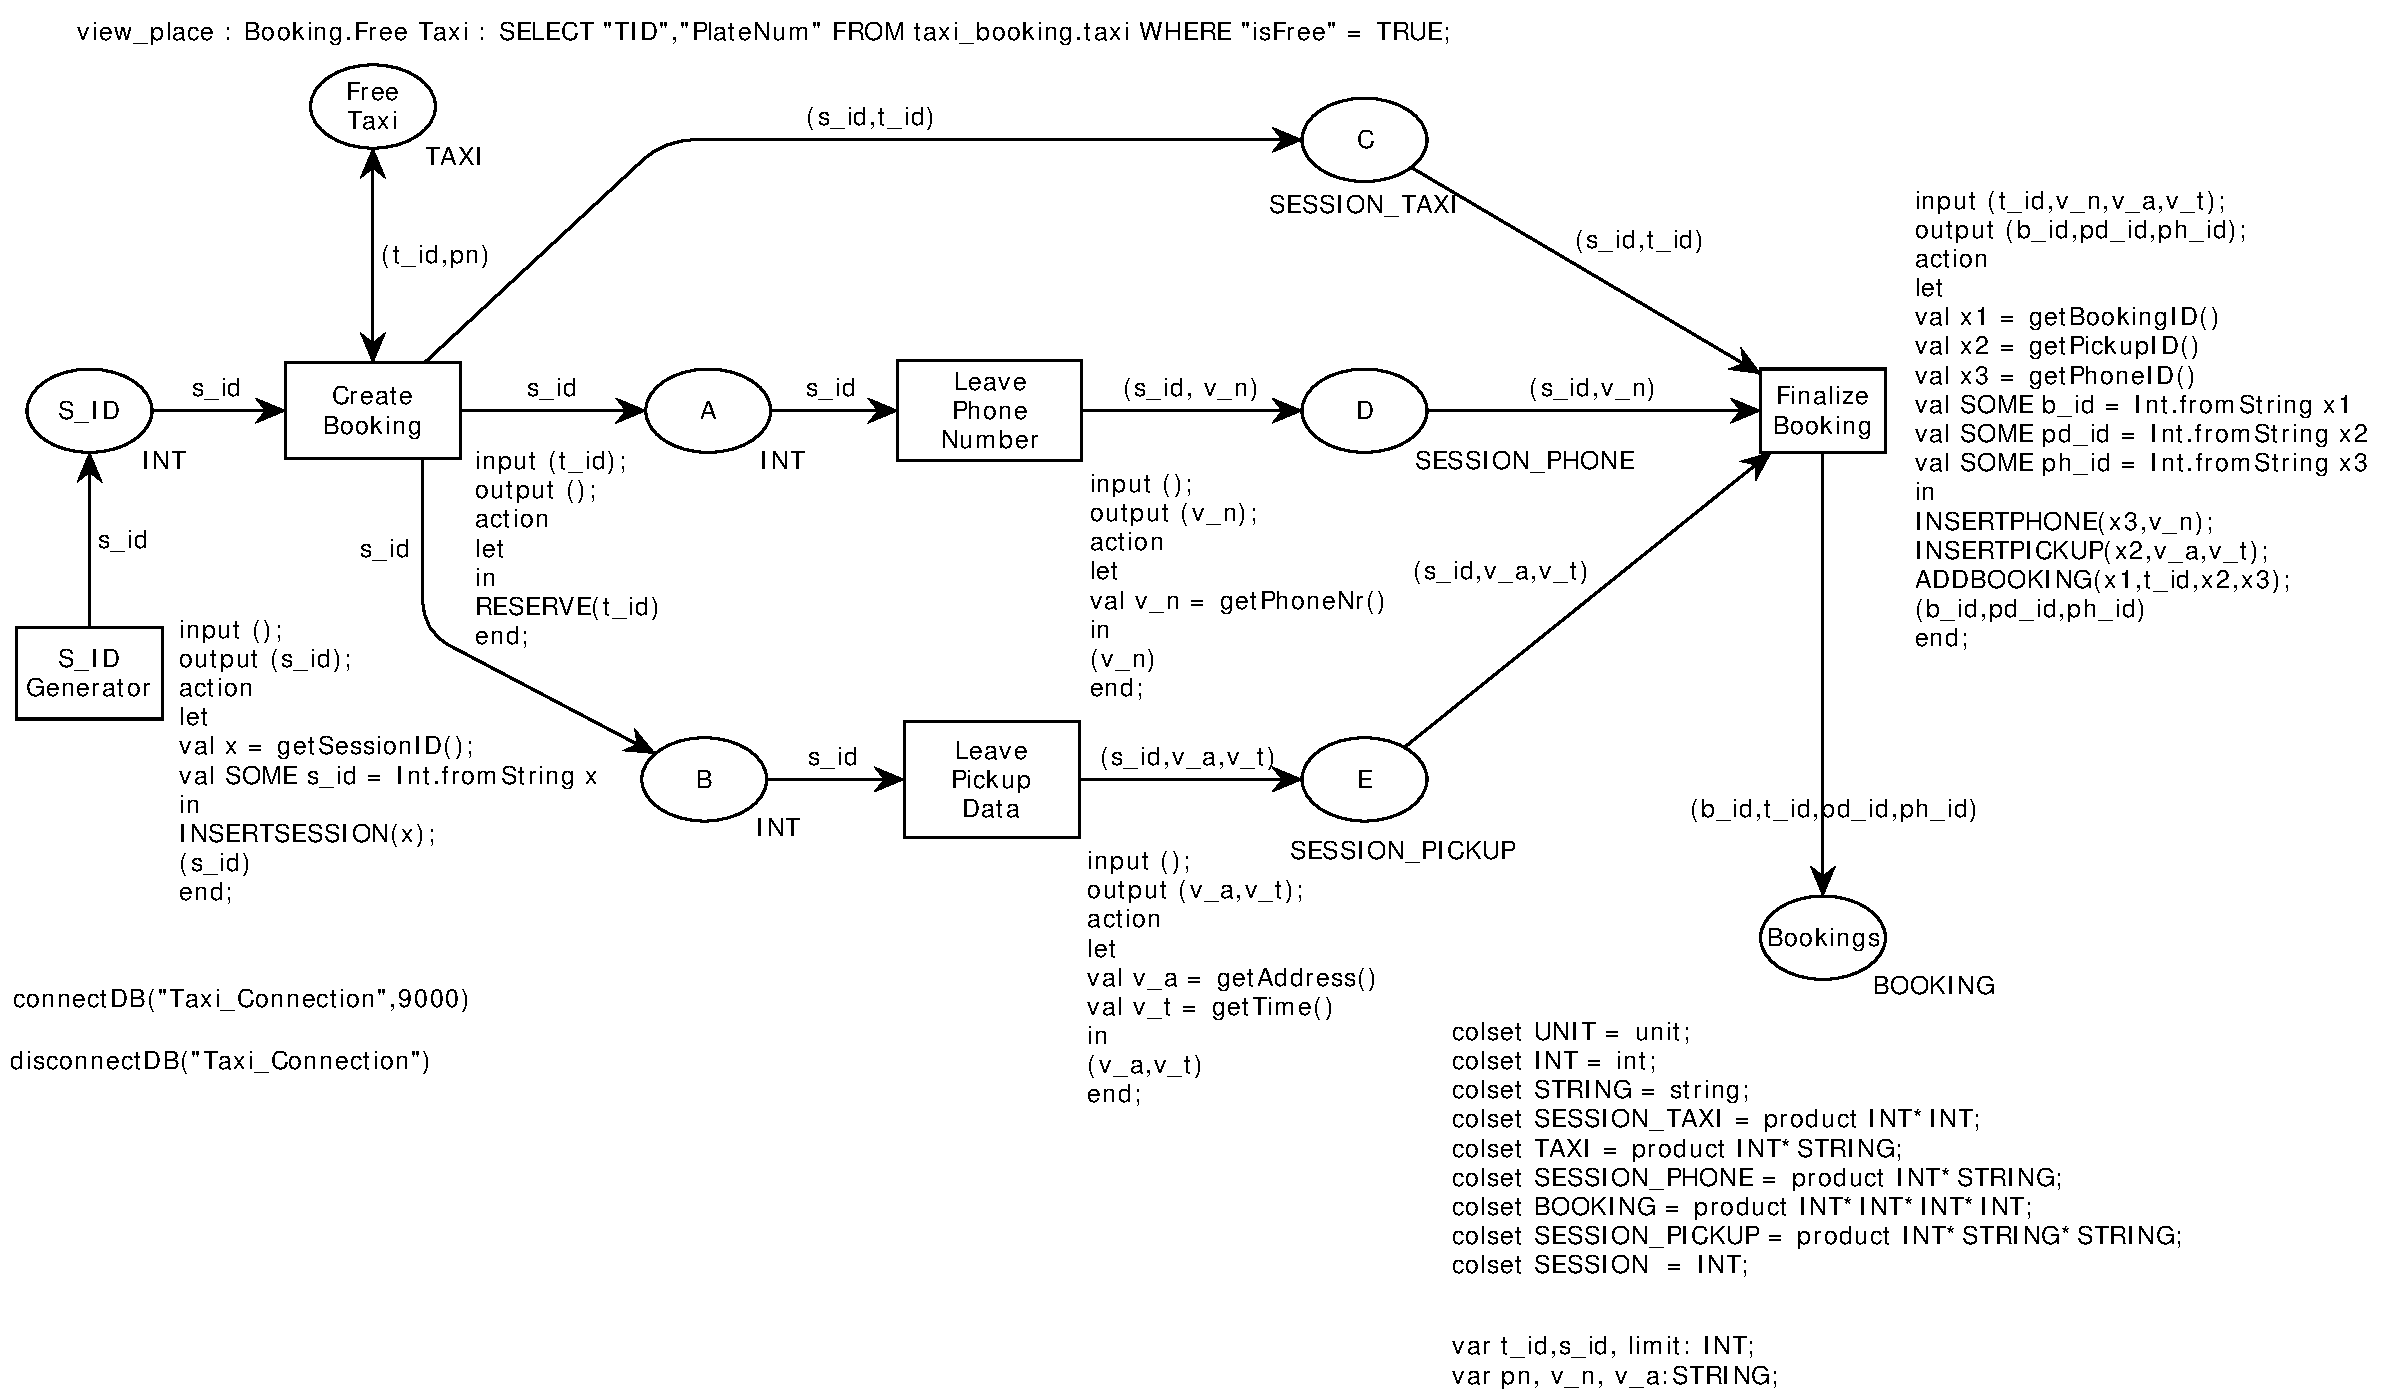
\includegraphics[scale = 0.35]{DBN_Impl_executable_model.pdf}
%	\caption{Executable DB-net model for taxi booking}
%	\label{fig:DBN_Impl_executable_model}
%\end{figure}
%
%\subparagraph*{\textnormal{In this model (see Figure \ref{fig:DBN_Impl_executable_model}), a session id generator (transition \textit{S\_ID Generator}) is attached which queries the \textit{session} table and generates an unique identifier for the table. The fresh variables generated by this transition is \textit{s\_id}. The \textit{action} part of \textit{S\_ID Generator} transition is: }}
%
%\subparagraph*{}
%\begin{lstlisting}[showstringspaces=false, language = ML, caption = Action part of transition : S\_ID Generator, captionpos=b, label = lst:DBN_Impl_action_sid_gen, numbers=left,
%stepnumber=1]
%let
%val x = getSessionID();
%val SOME s_id = Int.FromString x
%in
%INSERTSESSION(x);
%(s_id)
%end;
%\end{lstlisting}
%
%\subparagraph*{\textnormal{Functions \textit{getSessionID} and \textit{INSERTSESSION} are ML functions. \textit{getSessionID} generates a six digit unique session id for the \textit{session} table whereas \textit{INSERTSESSION} inserts the generated session id to the \textit{session} table. These ML functions can be defined as: }}
%
%\subparagraph*{}
%\begin{lstlisting}[showstringspaces=false, language = ML, caption = Functions for generating and inserting session ID, captionpos=b, label = lst:DBN_Impl_session_func,numbers=left,
%stepnumber=1]
%fun getSessionID() = getFromDB("taxi_booking.session","\"SID\"","genUniqueID","6");
%fun INSERTSESSION(s_id) = exQuery("exQuery","INSERT INTO taxi_booking.session VALUES ("^ s_id ^ ");" );
%\end{lstlisting}
%
%\subparagraph*{\textnormal{In Listing \ref{lst:DBN_Impl_action_sid_gen}, in line 2, variable \textit{x} stores the generated session ID from the \textit{getSessionID} function. In the DB-nets model the variable \textit{s\_id} is defined as \textit{integer}, hence we need to convert \textit{x} to \textit{integer}\footnote{The data type of the variable \textit{x} is \textit{string}, because it is returned from the function which uses Comms/CPN APIs which returns string.}. In line 6, the variable \textit{s\_id} is returned as the output variable.}}
%
%\subparagraph*{\textnormal{Let's take another example of the transition \textit{LEAVE PHONE NUMBER} where the data acquisition takes place without consulting the database. The \textit{action} part in this transition is defined as:}}
%
%\subparagraph*{}
%\begin{lstlisting}[showstringspaces=false, language = ML, caption = Action part of transition : LEAVE PHONE NUMBER, captionpos=b, label = lst:DBN_Impl_action_leave_ph_number, numbers=left,
%stepnumber=1]
%let
%val v_n = getPhoneNr()
%in
%(v_n)
%end;
%\end{lstlisting}
%
%\subparagraph*{\textnormal{In Listing \ref{lst:DBN_Impl_action_leave_ph_number}, the ML function \textit{getPhoneNr} internally calls \textit{getRandom} function which returns a randomly generated phone number of a fixed length. The ML definition of \textit{getPhoneNr} and \textit{getRandom} is:}}
%
%\subparagraph*{}
%\begin{lstlisting}[showstringspaces=false, language = ML, caption = Functions for acquiring phone number, captionpos=b, label = lst:DBN_Impl_getPhone_func]
%fun getPhoneNr()= getRandom("randomInt","10");
%\end{lstlisting}
%
%\subparagraph*{\textnormal{In Listing \ref{lst:DBN_Impl_action_leave_ph_number}, in line 2, the variable \textit{v\_n} acquires the ten digit phone number from the function \textit{getPhoneNr}. Similarly, for transition like \textit{Leave Pickup Data}, we could use different flavours of \textit{getRandom} function such as \textit{randomString} or \textit{randomTime}\footnote{for randomTime, one should always fix the length to 6, which signifies hh::mm::ss in the time format.}. The function for \textit{Leave Phone Number} transition is defined as follows:}}
%
%\subparagraph*{}
%\begin{lstlisting}[showstringspaces=false, language = ML, caption = Functions for acquiring address and time, captionpos=b, label = lst:DBN_Impl_add_time_func]
%fun getAddress() = getRandom("randomString","20");
%fun getTime() = getRandom("randomTime", "6");
%\end{lstlisting}
%
%
%\subparagraph*{\textnormal{Now we are aware about the modelling and execution of DB-nets in CPN Tools. If the reader is interested in more detailed and low level implementation of the extension, then one could read refer {\color{red}documentation link}. In the next chapter we will look at analysis on DB-nets.}}
%%\end{comment}

